\documentclass[11pt]{article}
\usepackage[T1]{fontenc}
\usepackage[utf8]{inputenc}
\usepackage{amsmath,amssymb,amsthm,mathtools,xparse,enumitem,hyperref,tikz,pgfplots}
\pgfplotsset{compat=1.18}
\usepackage[a4paper,margin=25mm]{geometry}
\numberwithin{equation}{section}
\newtheorem{theorem}{Theorem}[section]
\newtheorem{proposition}[theorem]{Proposition}
\newtheorem{lemma}[theorem]{Lemma}
\newtheorem{corollary}[theorem]{Corollary}
\theoremstyle{definition}
\newtheorem{definition}[theorem]{Definition}
\newtheorem{example}[theorem]{Example}
\newtheorem{examples}[theorem]{Examples}
\newtheorem{problem}[theorem]{Problem}
\theoremstyle{remark}
\newtheorem{remark}[theorem]{Remark}
\renewcommand{\theoremautorefname}{Result}
\newcommand{\pqty}[1]{\left(#1\right)}
\newcommand{\bqty}[1]{\left[#1\right]}
\newcommand{\Bqty}[1]{\left\{#1\right\}}
\newcommand{\abs}[1]{\left|#1\right|}
\newcommand{\norm}[1]{\left\lVert#1\right\rVert}
\newcommand{\flatfrac}[2]{\frac{#1}{#2}}
\newcommand{\set}[2]{\left\{#1\mid #2\right\}}
\newcommand{\ccintv}[2]{[#1,#2]}
\newcommand{\oointv}[2]{(#1,#2)}
\newcommand{\functiondomain}[3]{#1:#2\to #3}
\newcommand{\function}[5]{#1:#2\to #3,\quad #4\mapsto #5}
\newcommand{\pmqty}[1]{\begin{pmatrix}#1\end{pmatrix}}
\NewDocumentCommand{\vb}{s m}{\IfBooleanTF{#1}{\boldsymbol{#2}}{\mathbf{#2}}}
\newcommand{\RR}{\mathbb{R}}
\newcommand{\ZZ}{\mathbb{Z}}
\newcommand{\transpose}{^{\mathsf{T}}}
\newcommand{\inverse}{^{-1}}
\newcommand{\grad}{\nabla}
\newcommand{\vdot}{\cdot}
\newcommand{\cross}{\times}
\newcommand{\curl}{\nabla\times}
\renewcommand{\div}{\nabla\cdot}
\newcommand{\unitv}[1]{\widehat{\mathbf{#1}}}
\newcommand{\levicivita}{\varepsilon}
\newcommand{\bigO}{\mathcal{O}}
\newcommand{\contClass}[1]{C^{#1}}
\newcommand{\smoothClass}{C^\infty}
\newcommand{\contClassSymb}{\mathcal{C}}
\newcommand{\legendre}[1]{{#1}^{*}}
\newcommand{\llegendre}[1]{{#1}^{**}}
\newcommand{\rightbar}[1]{\left.#1\right|}
\newcommand{\qand}{\quad\text{and}\quad}
\newcommand{\qqtext}[1]{\quad\text{#1}\quad}
\DeclareMathOperator{\dom}{dom}
\DeclareMathOperator{\tr}{tr}
\DeclareMathOperator{\sign}{sgn}
\DeclareMathOperator{\diag}{diag}
\newcommand{\dimM}{\mathsf M}
\newcommand{\dimL}{\mathsf L}
\newcommand{\dimT}{\mathsf T}
\NewDocumentCommand{\dd}{o m}{\,\mathrm{d}\IfNoValueF{#1}{^{#1}}#2}
\NewDocumentCommand{\var}{o m}{\delta\IfNoValueF{#1}{^{#1}}#2}
\newcommand{\fdv}[2]{\frac{\delta #1}{\delta #2}}
\NewDocumentCommand{\dv}{s o m g}{\IfNoValueTF{#4}{\frac{\mathrm{d}\IfNoValueF{#2}{^{#2}}}{\mathrm{d}#3\IfNoValueF{#2}{^{#2}}}}{\IfNoValueTF{#2}{\frac{\mathrm{d}#3}{\mathrm{d}#4}}{\frac{\mathrm{d}^{#2}#3}{\mathrm{d}#4^{#2}}}}}
\NewDocumentCommand{\pdv}{s o m g g}{\IfNoValueTF{#4}{\frac{\partial\IfNoValueF{#2}{^{#2}}}{\partial #3\IfNoValueF{#2}{^{#2}}}}{\IfNoValueTF{#5}{\IfNoValueTF{#2}{\frac{\partial #3}{\partial #4}}{\frac{\partial^{#2} #3}{\partial #4^{#2}}}}{\frac{\partial^2 #3}{\partial #4\,\partial #5}}}}
\title{Variational Principles: Convexity, Mechanics and the Calculus of Variations}
\author{Notes by Eason Shao; lectures by H. S. Reall}
\date{Cambridge Part IB, Easter Term 2026; revised 2026-09-28}
\begin{document}
\maketitle
\paragraph{Provenance and scope.}
Revised unofficial notes, not endorsed by the lecturer. Source: Eason Shao,
\texttt{ib-damtp-variational-principles-et-2026}. The twelve substantive chapters
and original credits are retained. Missing personal-package macros are defined locally.
Selected mathematical errors, hypotheses and proofs have been corrected; this is not an
exhaustive certification. Raster illustrations are replaced by mathematical descriptions.
Keep hypotheses, statements and their proofs linked when forming retrieval units.
\paragraph{Conventions.}
Bold symbols denote vectors; \(\vb v^2=\vb v\cdot\vb v\), and \(|\vb v|\) denotes
the Euclidean norm. Repeated indices are summed where stated. \(f^*\) denotes the
convex conjugate and \(f^{**}\) the biconjugate. In this course the symbol
\(\delta^2F[y,\xi]\) denotes the coefficient of \(\epsilon^2\) in
\(F[y+\epsilon\xi]\), hence one half of the second directional derivative.
Stationarity does not by itself establish a minimum or maximum.
\tableofcontents
\section*{Introduction}

The motivational problem of this course is the following.

\begin{problem}[Shortest Path Problem]\label{variation-unit-0001}
    \label{prob:shortest-path}%
    How do we find the shortest path between two points:
    \begin{enumerate}
        \item in Euclidean Space;
        \item on the Sphere;
        \item on a general curved surface, e.g., potato?
    \end{enumerate}
\end{problem}

In problem (i), we may write the path in the form \(y = y\pqty{x}\), with \(a \leq x \leq b\). Then its length is given by
\[
    L \bqty{y} = \int_{a}^{b} \sqrt{1 + y'^2} \dd{x}.
\]

We can find the length of a parametrised curve similarly in (ii) and (iii).

This is a \emph{functional}, which is a map from a function to a number, and the goal is to find the choice of the function \(y\pqty{x}\) that minimises this functional. We will develop tools in this course to determine minima/maxima  of functionals.

\section{Calculus on \(\RR^n\)}

Consider \(\functiondomain{f}{\RR^n}{\RR}\), and we write
\[
    \vb{x} = \pqty{x_1, x_2, \ldots, x_n} \in \RR^n.
\]

Assume \(f\) is sufficiently differentiable (and in particular, at least \(\contClass{2}\), meaning \(f\) is twice continuously differentiable).

\begin{definition}[Stationary Point]\label{variation-unit-0002}
    \label{def:stationary-point}%
    We say a point \(\vb{a} \in \RR^n\) is a \emph{stationary point} of \(f\), if
    \[
        \pqty{\grad f} \pqty{\vb{a}} = \vb{0},
    \]
    where the \emph{gradient} is given by
    \[
        \grad f = \pqty{\pdv{f}{x_1}, \pdv{f}{x_2}, \ldots, \pdv{f}{x_n}}.
    \]
\end{definition}

We may also Taylor expand a function about a point, having
\[
    f\pqty{\vb{x}} = f\pqty{\vb{a}} + \sum_{i} \pqty{x_i - a_i} \pqty{\nabla_i f} \pqty{\vb{a}} + \frac{1}{2} \sum_{i, j} \pqty{x_i - a_i} \pqty{x_j - a_j} H_{ij} \pqty{\vb{a}} + o\pqty{\norm{\vb{x} - \vb{a}}^2},
\]
where the \emph{Hessian matrix} is given by
\[
    H_{ij} = \pdv{f}{x_i}{x_j}.
\]

Since \(f\) is \(\contClass{2}\), \(H_{ij} = H_{ji}\). From now on, we simplify the notation with \(\vb{a} = \vb{0}\) by a translation to the origin. Under the summation convention, at a stationary point, we have
\[
    f\pqty{\vb{x}} - f\pqty{\vb{0}} = \frac{1}{2} x_i H_{ij} x_j + o\pqty{\abs{\vb{x}}^2}.
\]

Recall that we may diagonalise \(H_{ij}\), since it is symmetric, and we may rotate the coordinates under the transformation
\[
    x_i = R_{ij} x'_{j}.
\]

Then the new Hessian matrix will be transformed as
\[
    \vb{H}' = \vb{R}\transpose \vb{H} \vb{R} = \diag(\lambda_1,\lambda_2,\ldots,\lambda_n)
\]
and the eigenvalues \(\lambda_1, \ldots, \lambda_n\) are the eigenvalues of \(\vb{H}\). Note that since \(\vb{H}\) is real, symmetric, all the eigenvalues are therefore real.

After diagonalisation, the quadratic form will be diagonalised as
\[
    f\pqty{\vb{x}} - f\pqty{\vb{0}} = \frac{1}{2} \sum_{i = 1}^{n} \lambda_i x_i'^2 + o\pqty{\abs{\vb{x}}^2}.
\]

Therefore, we have the following result.

\begin{proposition}[Classification of Stationary Point using Hessian Matrix]\label{variation-unit-0003}
    \label{prop:classification-stationary-point}%
    Using the Hessian matrix, at a stationary point,
    \begin{itemize}
        \item if \(\lambda_i > 0\) for all \(i\), then \(f\pqty{\vb{x}} > f\pqty{\vb{0}}\) for sufficiently small nonzero \(\vb{x}\), and hence \(\vb{x} = \vb{0}\) is a \emph{local minimum};
        \item if \(\lambda_i < 0\) for all \(i\), then \(\vb{x} = \vb{0}\) is a \emph{local maximum};
        \item if there is some \(\lambda_i > 0\) and some other \(\lambda_j < 0\), then \(\vb{x} = \vb{0}\) is a \emph{saddle point}.
    \end{itemize}
\end{proposition}

\begin{remark}\label{variation-unit-0004}
    The remaining cases are \emph{degenerate} stationary points -- the quadratic test is inconclusive; higher-order behaviour must be examined.
\end{remark}

\begin{corollary}[Hessian Matrix in Two-Variable Case]\label{variation-unit-0005}
    \label{cor:hessian-2-d}%
    In the special case where \(n = 2\), we have
    \begin{itemize}
        \item if \(\det \vb{H} > 0\) and \(\tr \vb{H} > 0\), then it is a local minimum;
        \item if \(\det \vb{H} > 0\) and \(\tr \vb{H} < 0\), then it is a local maximum;
        \item if \(\det \vb{H} < 0\), then it is a saddle point;
        \item if \(\det \vb{H} = 0\), then it is degenerate.
    \end{itemize}
\end{corollary}

\begin{proof}
    We have \(\det \vb{H} = \lambda_1 \lambda_2\), and \(\tr \vb{H} = \lambda_1 + \lambda_2\). Applying \autoref{prop:classification-stationary-point} gives the result.
\end{proof}

\begin{remark}\label{variation-unit-0006}
    If a local minimum is not a global minimum, then either:
    \begin{itemize}
        \item there is another stationary point that is the global minimum; or
        \item the global minimum occurs on the boundary of the domain of \(f\); or
        \item \(f\) does not have a global minimum.
    \end{itemize}
\end{remark}

\begin{example}[Finding and Classifying Stationary Points]\label{variation-unit-0007}
    \label{ex:finding-classifying-stationary-points}%
    Consider the function \(\functiondomain{f}{\RR^2}{\RR}\), given by
    \[
        f\pqty{x, y} = x^3 + y^3 - 3xy.
    \]

    We find the gradient as
    \[
        \grad f = \pqty{3 x^2 - 3y, 3 y^2 - 3x},
    \]
    and note
    \[
        \grad f = \vb{0} \iff x^2 = y \text{ and } y^2 = x.
    \]

    This then solves to \(\pqty{x, y} = \pqty{0, 0}\) or \(\pqty{x, y} = \pqty{1, 1}\).

    Now, looking at the Hessian matrix, we have
    \[
        \vb{H} = \begin{pmatrix}
            6x & -3 \\ -3 & 6y
        \end{pmatrix}.
    \]

    The determinant and the trace are therefore given by
    \[
        \det \vb{H} = 9 \pqty{4xy - 1}, \quad \tr \vb{H} = 6 \pqty{x + y}.
    \]

    At \(\pqty{x, y} = \pqty{1, 1}\), \(\det \vb{H} = 27 > 0\) and \(\tr \vb{H} = 12 > 0\). Therefore, \(\pqty{1, 1}\) is a local minimum, and
    \[
        f\pqty{1, 1} = -1.
    \]

    At \(\pqty{x, y} = \pqty{0, 0}\), \(\det \vb{H} = -9 < 0\). Therefore, \(\pqty{0, 0}\) is a saddle, and
    \[
        f\pqty{0, 0} = 0.
    \]

    We may calculate the eigenvalues and the corresponding eigenvectors as
    \[
        \lambda_1 = -3, \quad \vb{e}_1 = \begin{pmatrix}
            1 \\ 1
        \end{pmatrix}
    \]
    and
    \[
        \lambda_2 = 3, \quad \vb{e}_2 = \begin{pmatrix}
            1 \\ -1
        \end{pmatrix}.
    \]

    Therefore, \(\pqty{0, 0}\) is a local maximum along the line parallel to \(\vb{e}_1\) (\(y = x\)), while it is a local minimum along the line parallel to \(\vb{e}_2\) (\(y = -x\)).

    But note \(f\) does not have a global maximum or minimum -- we can make \(x\) and \(y\) very large (but of the same sign), and \(f\) increases/decreases without bound.
\end{example}

\section{Convex Functions}
In the differentiable first- and second-order characterisations below, take the domain to be open and convex. The purely defining convexity inequalities also apply to non-open convex domains.

\begin{definition}[Convex Set]\label{variation-unit-0008}
    \label{def:convex-set}%
    A set \(S \subseteq \RR^n\) is \emph{convex}, if for any \(\vb{x}, \vb{y} \in S\) and \(t \in \ccintv{0}{1}\), we have
    \[
        t \vb{x} + \pqty{1 - t} \vb{y} \in S.
    \]
\end{definition}

\autoref{def:convex-set} says that a set is convex, if and only if the straight line segment that connects any two points are included in the set.

\begin{definition}[Graph of Function]\label{variation-unit-0009}
    \label{def:graph-of-fn}%
    Let \(f\) be a function with domain \(\dom\pqty{f} \subseteq \RR^n\), i.e., \(\functiondomain{f}{\dom\pqty{f}}{\RR}\). The \emph{graph} of \(f\) is the surface
    \[
        z = f\pqty{\vb{x}}
    \]
    in \(\RR^{n + 1}\), with coordinates \(\pqty{\vb{x}, z}\). A \emph{chord} of \(f\) is a line segment joining \(2\) points of its graph.
\end{definition}

\begin{definition}[Convex Function]\label{variation-unit-0010}
    \label{def:convex-function}%
    Let \(S=\dom(f)\). A function \(f\) is \emph{convex}, if
    \begin{itemize}
        \item its domain \(\dom\pqty{f}\) is convex (as a set); and
        \item the graph of \(f\) lies below, or on, its chords; mathematically, for any \(\vb{x}, \vb{y} \in S\) and \(t \in \ccintv{0}{1}\), we have
        \begin{equation}
            f\pqty{t \vb{x} + \pqty{1 - t} \vb{y}} \leq t f\pqty{\vb{x}} + \pqty{1 - t} f\pqty{\vb{y}}. \label{eq:convex-condition}
        \end{equation}
    \end{itemize}

    If instead, \autoref{eq:convex-condition} is strict: for any \(\vb{x}, \vb{y} \in S\) with \(\vb{x} \neq \vb{y}\), and \(t \in \oointv{0}{1}\), we have
    \begin{equation}
        f\pqty{t \vb{x} + \pqty{1 - t} \vb{y}} < t f\pqty{\vb{x}} + \pqty{1 - t} f\pqty{\vb{y}}, \label{eq:strict-convex-condition}
    \end{equation}
    then we say \(f\) is \emph{strictly convex}.

    We say \(f\) is \emph{(strictly) concave} if \(-f\) is (strictly) convex.
\end{definition}

Note that the first property is important, since we need the domain to be convex for \(f\pqty{t \vb{x} + \pqty{1 - t} \vb{y}}\) to be well-defined in the first place.

\begin{figure}[ht!]
    \centering
    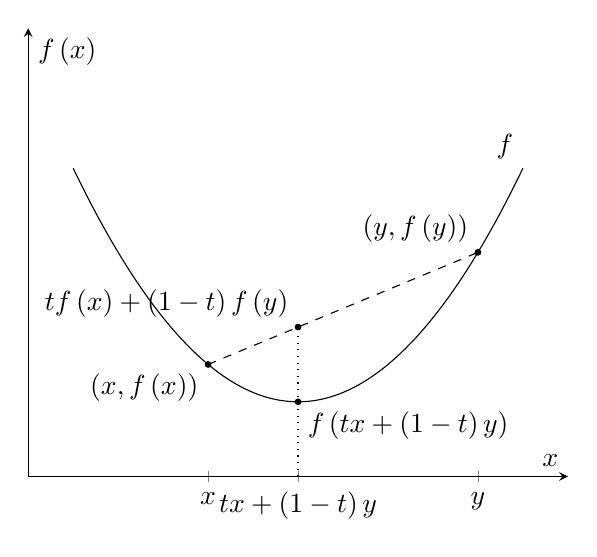
\begin{tikzpicture}
        \begin{axis}[
            axis lines = middle,
            xlabel = {\(x\)},
            ylabel = {\(f\pqty{x}\)},
            xmin = 0, xmax = 6,
            ymin = 0, ymax = 6,
            samples = 100,
            domain = 0.5:5.5,
            xtick = {2, 3, 5},
            xticklabels = {\(x\), \(t x+\pqty{1-t}y\), \(y\)},
            ytick = \empty
        ]

            \addplot[no marks] {0.5*(x-3)^2 + 1};
            \node[above left] at (axis cs:5.5,4.125) {\(f\)};

            \addplot[only marks, mark=*, mark size=1pt]
                coordinates {(2, 1.5) (5, 3)};

            \node[below left] at (axis cs:2, 1.5) {\(\pqty{x, f\pqty{x}}\)};
            \node[above left] at (axis cs:5, 3) {\(\pqty{y, f\pqty{y}}\)};

            \addplot[dashed] coordinates {(2, 1.5) (5, 3)};
            \addplot[only marks, mark=*, mark size=1pt]
                coordinates {(3, 2) (3, 1)};
            \node[above left] at (axis cs:3, 2) {\(t f\pqty{x} + \pqty{1 - t} f\pqty{y}\)};
            \node[below right] at (axis cs:3, 1) {\(f\pqty{t x + \pqty{1 - t} y}\)};

            \addplot[dotted] coordinates {(3, 0) (3, 2)};

        \end{axis}
    \end{tikzpicture}

    \caption{Convex Function}
    \label{fig:convex-fn}
\end{figure}

\begin{examples}[Convex Functions]\label{variation-unit-0011}
    \label{ex:convex-fn}%
    \begin{enumerate}
        \item The function \(f\pqty{x} = x^2\) is strictly convex, since
        \[
            \bqty{\pqty{1 - t} x + ty}^2 - \pqty{1 - t} x^2 - t y^2 = - t \pqty{1 - t} \pqty{x - y}^2 < 0
        \]
        for \(t \in \oointv{0}{1}\), \(x \neq y\).

        \item The functions \(f\pqty{x} = e^x\) and \(g\pqty{x} = e^{-x}\) are strictly convex.
        
        \item The function \(f\pqty{x} = \abs{x}\) is convex but not strictly convex: to show it is not strict, take for example \(x = 1\) and \(y = 2\), because some chords lie on the graph.
    \end{enumerate}
\end{examples}

\subsection{First Order Conditions}

\begin{theorem}[First Order Condition]\label{variation-unit-0012}
    \label{thm:first-order-condition}%
    If \(f\) is differentiable, then \autoref{eq:convex-condition} is equivalent to
    \begin{equation}
        \forall \vb{x}, \vb{y} \in \dom\pqty{f}: f\pqty{\vb{y}} \geq f\pqty{\vb{x}} + \pqty{\vb{y} - \vb{x}} \vdot \grad f\pqty{\vb{x}} \label{eq:first-order-condition}
    \end{equation}

    Geometrically, this means that the graph of \(f\) lies on or above any tangent plane, as shown in \autoref{fig:convex-fn-tangents} for the one-dimensional case.
\end{theorem}

\begin{figure}[ht!]
    \centering
    \begin{tikzpicture}
        \begin{axis}[
            axis lines = middle,
            xlabel = {\(x\)},
            ylabel = {\(f(x)\)},
            xmin = -1, xmax = 5,
            ymin = -2, ymax = 9,
            xtick = \empty,
            ytick = \empty,
            domain = 0:4,
            samples = 100,
            width = 10cm
        ]

            \addplot[no marks, thick, blue] {0.5*x^2};

            \addplot[only marks, mark=*, mark size = 1pt] coordinates {(1, 0.5) (2, 2) (3, 4.5)};

            \addplot[domain=0.25:4.5] {1 * (x - 1) + 0.5};
            \addplot[domain=0.4:4.2] {2 * (x - 2) + 2};
            \addplot[domain=0.5:4.1] {3 * (x - 3) + 4.5};
        \end{axis}
    \end{tikzpicture}

    \caption{Convex Function and its Tangents}
    \label{fig:convex-fn-tangents}
\end{figure}

\begin{corollary}[Convex Functions have Stationary Points as Global Minimums]\label{variation-unit-0013}
    \label{cor:stationary-point-global-minimum}%
    If \(f\) is convex and differentiable, then any stationary point is a global minimum.
\end{corollary}

\begin{proof}
    If \(\vb{a}\) is a stationary point, \(\grad f\pqty{\vb{a}} = \vb{0}\), so \autoref{eq:first-order-condition} implies that \(f\pqty{\vb{y}} \geq f\pqty{\vb{a}}\), for all \(\vb{y} \in \dom\pqty{f}\).
\end{proof}

Now we prove the first-order condition.

\begin{proof}[\proofname\ that \autoref{eq:convex-condition} implies \autoref{eq:first-order-condition}]
    Let
    \[
        h\pqty{t} = \pqty{1 - t} f\pqty{\vb{x}} + t f\pqty{\vb{y}} - f\pqty{\pqty{1 - t} \vb{x} + t \vb{y}}.
    \]

    Then note that
    \[
        h'\pqty{0} = - f\pqty{\vb{x}} + f\pqty{\vb{y}} - \pqty{\vb{y} - \vb{x}} \vdot \grad f\pqty{\vb{x}}
    \]
    which is the difference of two sides in \autoref{eq:first-order-condition}.

    But note that by definition,
    \[
        h'\pqty{0} = \lim_{t \to 0^+} \frac{h\pqty{t} - h\pqty{0}}{t} = \lim_{t \to 0^+} \frac{h\pqty{t}}{t}.
    \]

    But note that \autoref{eq:convex-condition} gives that \(h\pqty{t} \geq 0\) for all \(t \in \oointv{0}{1}\), and hence \(h'\pqty{0} \geq 0\), giving \autoref{eq:first-order-condition}.
 
\end{proof}

\begin{proof}[\proofname\ that \autoref{eq:first-order-condition} implies \autoref{eq:convex-condition}]
    In this direction, note that \autoref{eq:first-order-condition} implies that
    \begin{align*}
        f\pqty{\vb{x}} &\geq f\pqty{\vb{z}} + \pqty{\vb{x} - \vb{z}} \vdot \grad f\pqty{\vb{z}} \\
        f\pqty{\vb{y}} &\geq f\pqty{\vb{z}} + \pqty{\vb{y} - \vb{z}} \vdot \grad f\pqty{\vb{z}}
    \end{align*}
    for all \(\vb{x}, \vb{y}\) and \(\vb{z} \in \dom\pqty{f}\).

    Taking a linear combination, we have
    \[
        \pqty{1 - t} f\pqty{\vb{x}} + t f \pqty{\vb{y}} \geq f\pqty{z} + \bqty{\pqty{1 - t} \vb{x} + t \vb{y} - \vb{z}} \vdot \grad f\pqty{\vb{z}}.
    \]

    We now choose \(\vb{z} = \pqty{1 - t} \vb{x} + t \vb{y}\), which implies \autoref{eq:convex-condition}.
\end{proof}

\begin{proposition}[Alternative First Order Condition]\label{variation-unit-0014}
    An alternative way to write \autoref{eq:first-order-condition} is that
    \begin{equation}
        \pqty{\vb{y} - \vb{x}} \vdot \pqty{\grad f\pqty{\vb{y}} - \grad f\pqty{\vb{x}}} \geq 0
        \label{eq:first-order-condition-alternative}
    \end{equation}
    for all \(\vb{x}, \vb{y} \in \dom\pqty{f}\).
\end{proposition}

In particular, for \(n = 1\), \autoref{eq:first-order-condition-alternative} states that \(\pqty{y - x} \pqty{f'\pqty{y} - f'\pqty{x}} \geq 0\), which implies \(f'\pqty{y} \geq f'\pqty{x}\) if \(y \geq x\), i.e., \(f'\) is monotonically increasing.

\begin{proof}[\proofname\ that \autoref{eq:first-order-condition} implies \autoref{eq:first-order-condition-alternative}]
    From \autoref{eq:first-order-condition}, we have
    \begin{align*}
        f\pqty{\vb{y}} &\geq f\pqty{\vb{x}} + \pqty{\vb{y} - \vb{x}} \vdot \grad f\pqty{\vb{x}}, \\
        f\pqty{\vb{x}} &\geq f\pqty{\vb{y}} + \pqty{\vb{x} - \vb{y}} \vdot \grad f\pqty{\vb{y}}.
    \end{align*}

    Adding these give \autoref{eq:first-order-condition-alternative}.
\end{proof}

\begin{proof}[\proofname\ that \autoref{eq:first-order-condition-alternative} implies \autoref{eq:first-order-condition}]
    We let \(\vb{z} = \pqty{1 - t} \vb{x} + t \vb{y}\).

    Then we have
    \begin{align*}
        f\pqty{\vb{y}} - f\pqty{\vb{x}} &= \bqty{f\pqty{\vb{z}}}_{t = 0}^{t = 1} \\
        &= \int_{0}^{1} \dd{t} \dv{t} f\pqty{\vb{z}} \\
        &= \int_{0}^{1} \dd{t} \pqty{\vb{y} - \vb{x}} \vdot \grad f\pqty{\vb{z}}.
    \end{align*}

    Hence,
    \[
        f\pqty{\vb{y}} - f\pqty{\vb{x}} - \pqty{\vb{y} - \vb{x}} \vdot \grad f\pqty{\vb{x}} = \int_{0}^{1} \dd{t} \Bqty{\pqty{\vb{y} - \vb{x}} \vdot \bqty{\grad f\pqty{\vb{z}} - \grad f \pqty{\vb{x}}}}.
    \]

    Replace \(\vb{y}\) with \(\vb{z}\) in \autoref{eq:first-order-condition-alternative} gives that \(t \Bqty{\cdots} \geq 0\) (by using that \(\vb{z} = \pqty{1 - t} \vb{x} + t \vb{y}\)), and hence \(\Bqty{\cdots} \geq 0\).

    Hence, the integral is non-negative, and \autoref{eq:first-order-condition} holds.
\end{proof}

\subsection{Second Order Condition}

\begin{theorem}[Second Order Condition]\label{variation-unit-0015}
    \label{thm:second-order-condition}%
    If \(f\) is \(\contClass{2}\), then \autoref{eq:convex-condition} is equivalent to all eigenvalues of the Hessian \(\vb{H} \pqty{\vb{x}}\) is non-negative, for all \(\vb{x} \in \dom\pqty{f}\). In other words, the Hessian is positive semi-definite.
\end{theorem}

\begin{proof}
For a convex \(C^2\) function and any direction \(v\),
\(f(x+hv)+f(x-hv)-2f(x)\ge0\). Divide by \(h^2\) and let \(h\to0\)
to obtain \(v^TH(x)v\ge0\). Conversely, along any line segment let
\(g(t)=f(x+t(y-x))\). Then \(g''(t)=(y-x)^TH(x+t(y-x))(y-x)\ge0\),
so \(g'\) is nondecreasing and \(g\) is convex. Its convexity inequality proves
convexity of \(f\) on the convex domain.
\end{proof}

\begin{example}[Using Second Order Conditions]\label{variation-unit-0016}
    Consider the function \(f\pqty{x, y} = \flatfrac{1}{xy}\), and \(\dom\pqty{f} = \set{\pqty{x, y}}{x > 0, y > 0}\). The Hessian is given by
    \[
        \vb{H} = \frac{1}{xy} \pmqty{\frac{2}{x^2} & \frac{1}{xy} \\ \frac{1}{xy} & \frac{2}{y^2}},
    \]
    and we have
    \[
        \det \vb{H} = \frac{3}{x^4 y^4} > 0
    \]
    and
    \[
        \tr \vb{H} = \frac{2}{xy} \pqty{\frac{1}{x^2} + \frac{1}{y^2}} > 0.
    \]

    This means the eigenvalues of \(\vb{H}\) are strictly positive in \(\dom\pqty{f}\), and hence \(f\) is strictly convex.

    Note that if we take the domain to be
    \[
        \dom\pqty{f} = \set{\pqty{x, y}}{xy > 0},
    \]
    it seems like \(f\) would still be convex -- but that is not the case, because \(\dom \pqty{f}\) is not convex, and hence \(f\) is not convex.
\end{example}

\section{Legendre Transform}

\subsection{Definition and Properties}

\begin{definition}[Legendre Transform]\label{variation-unit-0017}
    \label{def:legendre-transform}%
    The \emph{Legendre Transform} of \(\functiondomain{f}{\dom\pqty{f} \subseteq \RR^n}{\RR}\) is
    \[
        \legendre{f} \pqty{\vb{p}} = \sup_{\vb{x} \in \dom \pqty{f}} \bqty{\vb{p} \vdot \vb{x} - f\pqty{\vb{x}}}
    \]
    with its domain as \(\dom \pqty{\legendre{f}} = \set{\vb{p} \in \RR^n}{\text{the supremum exists and is finite}}\).
\end{definition}

\begin{proposition}[Legendre Transform is Convex]\label{variation-unit-0018}
    \label{prop:legendre-convex}%
    \(\legendre{f}\) is convex.
\end{proposition}

\begin{proof}
    Let \(\vb{p}, \vb{q} \in \dom \pqty{\legendre{f}}\), and \(t \in \oointv{0}{1}\). We note that
    \begin{align*}
        \sup_{\vb{x} \in \dom \pqty{f}} \Bqty{\bqty{\pqty{1 - t} \vb{p} + t \vb{q}} \cdot \vb{x} - f\pqty{\vb{x}}} &= \sup_{\vb{x} \in \dom \pqty{f}} \Bqty{\pqty{1 - t} \bqty{\vb{p} \vdot \vb{x} - f\pqty{\vb{x}}} + t \bqty{\vb{q} \vdot \vb{x} - f \pqty{\vb{x}}}} \\
        &\leq \pqty{1 - t} \sup_{\vb{x} \in \dom \pqty{f}} \pqty{\vb{p} \vdot \vb{x} - f\pqty{\vb{x}}} + t \sup_{\vb{x} \in \dom \pqty{f}} \pqty{\vb{q} \vdot \vb{x} - f\pqty{\vb{x}}}.
    \end{align*}

    Since the right-hand side is finite, so must be the left-hand side, and hence \(\pqty{1 - t} \vb{p} + t \vb{q} \in \dom \pqty{\legendre{f}}\). In particular, the previous inequality also showed that
    \[
        \legendre{f} \pqty{\pqty{1 - t} \vb{p} + t \vb{q}} \leq \pqty{1 - t} \legendre{f} \pqty{\vb{p}} + t \legendre{f} \pqty{\vb{q}}
    \]
    so \(\legendre{f}\) is indeed convex.
\end{proof}

\begin{proposition}\label{variation-unit-0019}
    \label{prop:dot-product-convex}%
    If \(f\) is convex, then so is
    \[
        F_{\vb{p}} \pqty{\vb{x}} = f\pqty{\vb{x}} - \vb{p} \vdot \vb{x}
    \]
    where \(\vb{p} \in \RR^n\) is fixed.
\end{proposition}

\begin{proof}
    We have \(\dom \pqty{F_{\vb{p}}} = \dom \pqty{f}\). Note
    \begin{align*}
        F_{\vb{p}} \pqty{\pqty{1 - t} \vb{x} + t \pqty{\vb{y}}} &= f\pqty{\pqty{1 - t} \vb{x} + t \vb{y}} - \vb{p} \vdot \pqty{\pqty{1 - t} \vb{x} + t \vb{y}} \\
        &\leq \pqty{1 - t} f \pqty{\vb{x}} + t f \pqty{\vb{y}} - \vb{p} \vdot \pqty{\pqty{1 - t} \vb{x} + t \vb{y}} \\
        &= \pqty{1 - t} F_{\vb{p}} \pqty{\vb{x}} + t F_{\vb{p}} \pqty{\vb{y}}.
    \end{align*}
\end{proof}

\begin{corollary}[Legendre Transform of convex functions]\label{variation-unit-0020}
    \label{cor:legendre-transform-of-convex-function}
    If \(f\) is convex and differentiable, then any stationary point of \(\vb{p} \vdot \vb{x} - f \pqty{\vb{x}}\) (which is a concave function, by \autoref{prop:dot-product-convex}) is a global maximum occurring at \(\vb{x} \pqty{\vb{p}}\) given by solving
    \begin{equation}
        \grad f\pqty{\vb{x}} = \vb{p}.
        \label{eq:legendre-transform-of-convex-function}
    \end{equation}

    Hence, we have
    \[
        \legendre{f} \pqty{\vb{p}} = \vb{p} \vdot \vb{x} \pqty{\vb{p}} - f\pqty{\vb{x} \pqty{\vb{p}}}.
    \]
\end{corollary}

\begin{remark}\label{variation-unit-0021}
    If \(f\) is \emph{strictly} convex, then any solution to \autoref{eq:legendre-transform-of-convex-function}, if it exists, is unique. The idea is to consider the chord joining the two maxima of the function, and use the concave version of \autoref{eq:strict-convex-condition}.
\end{remark}

\begin{examples}[Legendre Transforms for \(n = 1\)]\label{variation-unit-0022}
    \label{ex:legendre-one-dimensional}%
    \begin{enumerate}
        \item Consider the quadratic \(f\pqty{x} = \frac{1}{2} a x^2\) for \(a > 0\). \(f\) is strictly convex, and \autoref{eq:legendre-transform-of-convex-function} holds if and only if \(x = \flatfrac{p}{a}\). Hence,
        \[
            \legendre{f} \pqty{p} = \frac{p^2}{a} - \frac{p^2}{2a} = \frac{p^2}{2a}.
        \]
        
        This is indeed convex, with domain \(\RR\).

        \item Consider the function \(f\pqty{v} = - \sqrt{1 - v^2}\) defined for \(-1 < v < 1\). This is a semi-circle and is convex. \autoref{eq:legendre-transform-of-convex-function} holds if and only if \(p = \flatfrac{v}{\sqrt{1 - v^2}}\). This gives the solution
        \[
            v = \frac{p}{\sqrt{1 + p^2}}
        \]
        for \(p \in \RR\). Hence,
        \[
            \legendre{f} \pqty{p} = \frac{p^2}{\sqrt{1 + p^2}} + \frac{1}{\sqrt{1 + p^2}} = \sqrt{1 + p^2},
        \]
        and this is defined for \(p \in \RR\).

        \autoref{fig:graph-legendre-one-dimensional-2} are the graphs for the two functions.

        \item Let \(f\pqty{x} = cx\) for \(c > 0\). This is a convex function, but not strictly convex. The domain is given by \(\dom\pqty{f} = \RR\), and note
        \[
            px - f\pqty{x} = \pqty{p - c} x.
        \]

        If \(p \neq c\), the supremum of this is infinite (since \(x\) can be arbitrarily large in both directions). This supremum only exists for \(p = c\), and hence
        \[
            \legendre{f}\pqty{p} = 0
        \]
        only defined for \(p = c\), i.e. \(\dom \pqty{\legendre{f}} = \Bqty{c}\).
    \end{enumerate}
\end{examples}

\begin{figure}[ht!]
    \centering
    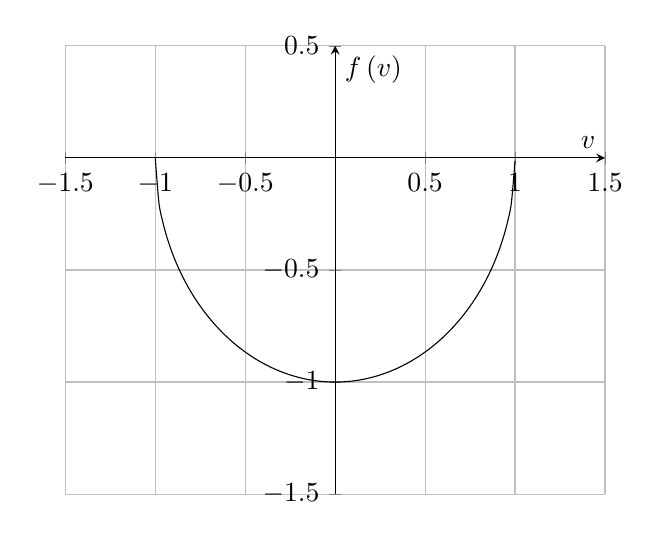
\begin{tikzpicture}[scale=1]
        \begin{axis}[grid=both,
                     xmin=-1.5, xmax=1.5, xlabel=\(v\),
                     ymin=-1.5, ymax=0.5, ylabel=\(f\pqty{v}\),
                    axis lines=center, >=stealth]
        \addplot[domain=-1:1, samples=100] plot[smooth] {- sqrt(1 - x^2)};
        \end{axis}
    \end{tikzpicture}


    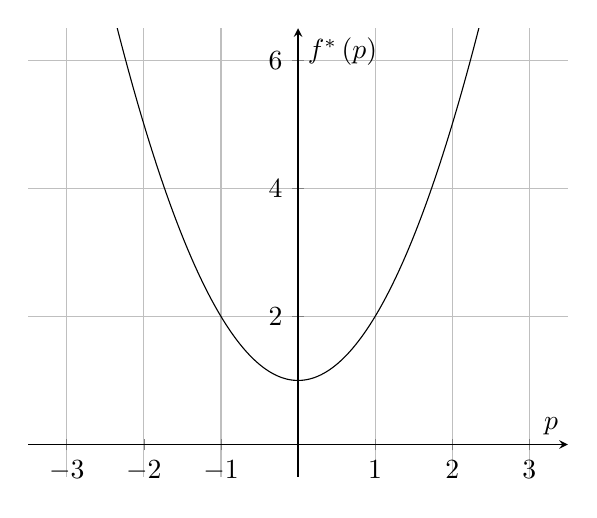
\begin{tikzpicture}[scale=1]
        \begin{axis}[grid=both,
                     xmin=-3.5, xmax=3.5, xlabel=\(p\),
                     ymin=-0.5, ymax=6.5, ylabel=\(\legendre{f}\pqty{p}\),
                    axis lines=center, >=stealth]
        \addplot[domain=-3:3, samples=100] plot[smooth] {sqrt{1 + x^2}};
        \end{axis}
    \end{tikzpicture}
    \caption{Graph for \autoref{ex:legendre-one-dimensional} (2)}
    \label{fig:graph-legendre-one-dimensional-2}
\end{figure}

What happens if we do a Legendre transform twice?

\begin{theorem}[Biconjugacy on the original open convex domain]\label{variation-unit-0023}
\label{thm:legendre-transform-of-legendre-transform}
Let \(f\) be differentiable and convex on a nonempty open convex set \(D\).
Then \(f^{**}(x)=f(x)\) for every \(x\in D\). This statement does not assert
that the effective domains of \(f\) and \(f^{**}\) are identical.
\end{theorem}
\begin{proof}
For every \(p\), the definition gives \(f^*(p)\ge p\cdot x-f(x)\), hence
\(f^{**}(x)\le f(x)\). Choose \(p=\nabla f(x)\). The supporting inequality
\(f(z)\ge f(x)+p\cdot(z-x)\) for all \(z\in D\) shows
\(f^*(p)=p\cdot x-f(x)\), proving the reverse inequality.
No inverse or differentiability of \(\nabla f\) is needed.
\end{proof}
\begin{remark}\label{variation-unit-0024}
Domain equality is not automatic. For \(f=0\) on \((0,1)\),
\(f^*(p)=\max(0,p)\), so \(f^{**}=0\) on \([0,1]\) and \(+\infty\) outside.
This follows directly by taking the supremum of \(px-\max(0,p)\).
\end{remark}

\begin{example}[Double Legendre Transform of the Line]\label{variation-unit-0025}
    We note that
    \[
        \llegendre{f} \pqty{x} = \sup_{p \in \Bqty{c}} \pqty{xp - \legendre{f} \pqty{p}} = cx = f\pqty{x}
    \]
    indeed.
\end{example}

\subsection{Application of Legendre Transforms in Thermodynamics}

An important application of Legendre transforms is in thermodynamics.

Consider a system made of many molecules (say \(10^{23}\)). We are concerned with the \emph{macroscopic} behaviour of the system, i.e., involving length scale \(\gg\) separation of molecules.

In \emph{thermal equilibrium}, we may describe the macroscopic physics of the system by just a few quantities: total energy \(E\), volume \(V\), temperature \(T\), pressure \(p\), and perhaps some others.

An \emph{isolated system} is one which is simply not interacting with anything else, for example a gas in a vacuum flask.

For a simple compressible system with fixed particle number and composition, in thermal equilibrium, macroscopic physics in gas in a vacuum flask is \textbf{fully specified} by two quantities, \(E\) and \(V\). However, microscopically, this is far away from the description in microscopic physics (since we need to specify the position, velocity, orientation, etc. of each microscopic molecule). Therefore, there is some number of \(\Omega \pqty{E, V}\) of microscopic configurations that ``look identical'' macroscopically, at the scale of
\[
    \Omega \sim 10^{10^{23}}
\]

\begin{definition}[Entropy]\label{variation-unit-0026}
    We define the \emph{entropy} as
    \begin{equation}
        \label{eq:entropy}%
        S\pqty{E, V} = k_{\text{B}} \log \Omega \pqty{E, V},
    \end{equation}
    where \(k_{\text{B}} = 1.380649\times10^{-23}\,\mathrm{J\,K^{-1}}\) is the Boltzmann constant.
\end{definition}

On the positive-temperature branch considered here, \((\partial S/\partial E)_V=1/T>0\). Thus entropy is locally strictly increasing with energy, allowing local inversion to define
\begin{equation}
    \label{eq:energy}%
    E = E \pqty{S, V}.
\end{equation}

\begin{definition}[Temperature, Pressure]\label{variation-unit-0027}
    We may define the \emph{temperature} and \emph{pressure} as
    \begin{subequations}
        \label{eq:temperature-pressure}%
        \begin{equation}
            \label{eq:temperature}%
            T = \pqty{\pdv{E}{S}}_{V} > 0
        \end{equation}
        \begin{equation}
            \label{eq:pressure}%
            P = - \pqty{\pdv{E}{V}}_{S}
        \end{equation}
    \end{subequations}
    respectively.
\end{definition}

\begin{proposition}[Fundamental Thermodynamic Relation]\label{variation-unit-0028}
    We have
    \begin{equation}
        \label{eq:fundamental-thermodynamic-relation}%
        \dd{E} = T \dd{S} - P \dd{V}
    \end{equation}
\end{proposition}

What is below is an overview of the Legendre Transforms -- details can be found on Example Sheets.

\begin{example}[Legendre Transforms for Temperature -- Helmholtz Free Energy]\label{variation-unit-0029}
    Now, we forget \autoref{eq:temperature} (for temperature). Consider the Legendre Transform of \(E\pqty{S, V}\) with respect to \(S\), with parameter \(T\). Call this \(-F\), i.e.,
    \[
        -F \pqty{T, V} = \sup_{S} \Bqty{TS - E \pqty{S, V}}.
    \] 

    We may show that the stability of equilibrium state implies that \(E\) is convex, with respect to \(S\). Now, \autoref{eq:legendre-transform-of-convex-function} maximises for \(S\pqty{T, V}\) satisfying \autoref{eq:temperature}, and
    \[
        F\pqty{T, V} = E - TS
    \]
    is called the \emph{Helmholtz Free Energy}.

    Note \autoref{eq:fundamental-thermodynamic-relation} implies that
    \[
        \dd{F} = - S \dd{T} - P \dd{V}
    \]
    and hence
    \begin{align*}
        S &= - \pqty{\pdv{F}{T}}_{V}, \\
        P &= - \pqty{\pdv{F}{V}}_{T}.
    \end{align*}

    In Part II, we will see that \(F\) is useful when considering an \emph{non-isolated} system in equilibrium with an \emph{environment} and temperature \(T\), for example gas in an uninsulated box.
\end{example}

\begin{example}[Legendre Transforms for Pressure -- Enthalpy]\label{variation-unit-0030}
    Similarly, we forget \autoref{eq:pressure} (for pressure). Consider the Legendre Transform of \(E\pqty{S, V}\) with respect to \(V\) at fixed \(S\), with parameter \(-P\). We call this \(-H\), i.e.,
    \[
        -H \pqty{S, P} = \sup_{V} \Bqty{-PV - E\pqty{S,V}}
    \]

    Similarly, applying \autoref{eq:legendre-transform-of-convex-function} maximises for \(V\) satisfying \autoref{eq:pressure}, and
    \[
        H\pqty{S, P} = E + PV
    \]
    is called the \emph{enthalpy}. It is very useful in chemistry.

    Now, \autoref{eq:fundamental-thermodynamic-relation} implies that
    \[
        \dd{H} = T \dd{S} + V \dd{P}
    \]
    and hence
    \begin{align*}
        T &= \pqty{\pdv{H}{S}}_{P}, \\
        V &= \pqty{\pdv{H}{P}}_{S}.
    \end{align*}
\end{example}

\begin{example}[Legendre Transforms for Both -- Gibbs Free Energy]\label{variation-unit-0031}
    Finally, we may take the Legendre transform of \(E \pqty{S, V}\) with respect to both \(S\) and \(V\) with parameters \(T, -P\), and call this \(-G\). Equivalently, with the same admissible thermodynamic states,
\(G(T,P)=\inf_V(F(T,V)+PV)=\inf_S(H(S,P)-TS)\).
These identities follow by taking the infimum of \(E-TS+PV\) successively in its two variables; a smooth equilibrium formula requires that the infimum be attained. We have
    \[
        -G \pqty{T, P} = \sup_{S, V} \Bqty{TS - PV - E \pqty{S, V}}
    \]
    and applying \autoref{eq:legendre-transform-of-convex-function}, we have the maximum of \(S\pqty{T, P}\) and \(V\pqty{T, P}\) gives both of \autoref{eq:temperature-pressure}. Hence, \(G\) is given by
    \[
        G\pqty{T, P} = E - TS + PV
    \]
    is called the \emph{Gibbs free energy}.

    Using \autoref{eq:fundamental-thermodynamic-relation} gives
    \[
        \dd{G} = -S \dd{T} + V \dd{P}
    \]
    and hence
    \begin{align*}
        S &= - \pqty{\pdv{G}{T}}_{P}, \\
        V &= \pqty{\pdv{G}{P}}_{T}.
    \end{align*}
\end{example}

\begin{definition}[Thermodynamic Potentials]\label{variation-unit-0032}
    \(E, F, G, H\) are called \emph{thermodynamic potentials}.
\end{definition}

Assuming that everything is \(\contClass{2}\), we have
\[
    \pdv{E}{S}{V} = \pdv{E}{V}{S},
\]
and hence
\[
    \pqty{\pdv{S} \pqty{\pdv{E}{V}}_S}_{V} = \pqty{\pdv{V} \pqty{\pdv{E}{S}}_{V}}_{S}.
\]

Applying \autoref{eq:temperature-pressure} gives
\[
    - \pqty{\pdv{P}{S}}_{V} = \pqty{\pdv{T}{V}}_{S}
\]

There are three similar equations that follow from doing the same steps with different thermodynamic potentials, from \(F, H\) and \(G\).

\begin{definition}[Maxwell Relations]\label{variation-unit-0033}
    The four equations derived from the four thermodynamic potentials are the \emph{Maxwell relations}.
\end{definition}

\section{Constraints and Lagrange Multipliers}

\subsection{Motivation}

Consider a smooth surface \(S\) in \(\RR^3\). If we have \(\functiondomain{f}{\RR^3}{\RR}\), how do we determine the maximum/minimum of \(f\) on \(S\)?

(A real-life example might be \(S\) is a hill, and \(f\) is the temperature scalar field, and we want to find which points on \(S\) are hottest/coldest.)

Let \(\pqty{u, v}\) parameterise \(S\), i.e., let
\[
    S: \quad \vb{x} = \vb{x} \pqty{u, v}
\]

We would like to optimise \(f\pqty{\vb{x} \pqty{u, v}}\).

But this is straightforward -- \(f\) is now effectively in terms of \(u\) and \(v\), so we want
\begin{align*}
    0 &= \pdv{u} f\pqty{\vb{x}} = \pqty{\grad f} \vdot \pqty{\pdv{\vb{x}}{u}}, \\
    0 &= \pdv{v} f\pqty{\vb{x}} = \pqty{\grad f} \vdot \pqty{\pdv{\vb{x}}{v}}.
\end{align*}

Recall from \textit{Vector Calculus} that the set
\[
    \Bqty{\pdv{\vb{x}}{u}, \pdv{\vb{x}}{v}}
\]
are linearly independent vectors tangent to \(S\). In other words, we have just shown \autoref{prop:max-min-of-function-on-surface} for a parametrisation of \(S\).

\begin{proposition}[Maximum/Minimum of Function on Surface]\label{variation-unit-0034}
    \label{prop:max-min-of-function-on-surface}%
    \(\vb{x}_0 \in S\) is a stationary point of \(f\) on \(S\), if and only if \(\grad f\pqty{\vb{x}_0}\) is normal to \(S\).
\end{proposition}

\subsection{Lagrange Multiplier with Single Constraint}
Assume the constraint is regular: \(\nabla g(x_0)\ne0\). Otherwise the multiplier equation need not capture every constrained stationary point.

In practice, we don't always have a nice explicit parametrisation \(\vb{x}\pqty{u, v}\) of \(S\), and more commonly, \(S\) is determined more implicitly of the form
\[
    g\pqty{\vb{x}} = 0
\]
where \(g\) is some other function on \(\RR^3\). This equation is called an \emph{constraint}, and the problem is to optimise \(f\) subject to the constraint \(g = 0\).

\begin{lemma}[Gradient is Perpendicular to Level Surface]\label{variation-unit-0035}
    \label{lem:gradient-perpendicular-level-surface}%
    \(\grad g\) is normal to the surface \(S\).
\end{lemma}

\begin{proof}
    Since \(g\pqty{\vb{x} \pqty{u, v}} = 0\), differentiating with respect to \(u\) and \(v\) just like above gives the result.
\end{proof}

So \autoref{prop:max-min-of-function-on-surface} is equivalent to
\[
    \grad f\pqty{\vb{x}_0} = \lambda \grad g\pqty{\vb{x}_0}
\]
for some \(\lambda\). Then, we want to solve this together with \(g\pqty{\vb{x}_0} = 0\) to find \(\vb{x}_0\) and \(\lambda\).

Note that \emph{both} equations are obtained by finding an \emph{unconstrained} stationary point of
\[
    \function{\phi}{\RR^4}{\RR}{\pqty{\vb{x}, \lambda}}{f\pqty{\vb{x}} - \lambda g\pqty{\vb{x}}.}
\]

Optimising with respect to \(\lambda\) recovers \(g\pqty{\vb{x}} = 0\), and optimising with respect to \(\vb{x}\) recovers \(\grad f = \lambda \grad g\), by differentiation.

\begin{definition}[Lagrange Multiplier]\label{variation-unit-0036}
    \label{def:lagrange-multiplier}%
    The \(\lambda\) defined above is a \emph{Lagrange multiplier}.
\end{definition}

Note whatever we did above generates to \(\RR^n\), but the difficulty is to determine the nature of the stationary points -- the relevant second-order form is the Hessian of the Lagrangian in the original variables, restricted to the tangent space of the constraints.

\begin{example}[Lagrnage Multiplier, Easier Example]\label{variation-unit-0037}
    Consider an open rectangular box with dimensions \(\pqty{x, y, z}\) (with the \(xy\) surface missing for the top). We want to minimise its surface area \(A\) subject to a constraint of fixed volume \(V = \flatfrac{L^3}{2}\).
        
    Mathematically,
    \[
        A = 2z \pqty{x + y} + xy
    \]
    with constraint
    \[
        xyz = \frac{L^3}{2}.
    \]

    A direct method could be eliminating the constraint by doing
    \[
        z = \frac{L^3}{2xy}
    \]
    and hence
    \[
        A = \frac{L^3}{x} + \frac{L^3}{y} + xy.
    \]

    Hence, \(A\) is stationary if and only if
    \[
        0 = \pdv{A}{x} = - \frac{L^3}{x^2} + y,
    \]
    and
    \[
        0 = \pdv{A}{y} = - \frac{L^3}{y^2} + x
    \]
    and hence \(x = y = L\), with \(z = \flatfrac{L}{2}\), and \(A = 3 L^2\).

    For \(x,y,L>0\), AM--GM gives \(L^3/x+L^3/y+xy\ge3L^2\), with equality exactly at \(x=y=L\); this certifies the global minimum.

    Using Lagrange multipliers, we consider the function
    \[
        \phi\pqty{x, y, z, \lambda} = A\pqty{x, y, z} - \lambda \pqty{xyz - \frac{L^3}{2}}.
    \]

    First, we look at
    \[
        0 = \pdv{\phi}{z} = 2\pqty{x + y} - \lambda xy,
    \]
    and this gives \(\lambda = \flatfrac{2 \pqty{x + y}}{xy}\).

    With respect to \(x\),
    \[
        0 = \pdv{\phi}{x} = 2z + y - \lambda yz = 2z + y - \frac{2 \pqty{x + y} z}{x} = \frac{y}{x} \pqty{x - 2z}.
    \]
    
    Hence, \(x = 2z\) or \(y = 0\), but we reject \(y = 0\) since it cannot satisfy the constraint.

    By symmetry, considering the \(y\) derivative gives \(y = 2z\).

    Finally, differentiating with respect to \(\lambda\), we have
    \[
        0 = \pdv{\phi}{\lambda} = -xyz + \frac{L^3}{2}
    \]
    recovering the constraint, so \(z = \flatfrac{L}{2}\) and \(x = y = L\).
\end{example}

The unrestricted Hessian in \((x,\lambda)\) does not classify the constrained
extremum. At a regular constrained stationary point use
\(d^T\nabla_x^2(f-\lambda g)d\) for tangent vectors \(d\), with
\(\nabla g\cdot d=0\). Indeed, for a feasible curve \(x(t)\), differentiating
\(g(x(t))=0\) twice and using \(\nabla f=\lambda\nabla g\) gives
\((f\circ x)''(0)=x'(0)^T\nabla_x^2(f-\lambda g)x'(0)\).
Definiteness of this restricted form supplies the usual sufficient local tests.

The main advantage of this method is it works even when the constraint is very complicated to solve explicitly (and often simpler even if the constraint can be solved).

\begin{example}[Optimising Quadratic Form]\label{variation-unit-0038}
    \label{ex:optimising-quadratic-form}%
    We find the minimum of the quadratic form on \(\RR^n\)
    \[
        f\pqty{\vb{x}} = x_i A_{ij} x_j
    \]
    on the surface \(\abs{\vb{x}}^2 = 1\), the unit sphere.

    We have
    \[
        \phi\pqty{\vb{x}, \lambda} = x_i A_{ij} x_j - \lambda \pqty{x_i x_i - 1}.
    \]

    Differentiating w.r.t. \(x_i\), we have (using product rule and removing a factor of 2) that
    \[
        0 = A_{ij} x_j - \lambda x_i.
    \]

    Differentiating w.r.t. \(\lambda\) recovers \(\abs{\vb{x}}^2 = 1\).

    We see that the stationary points are going to be the normalised eigenvectors of \(\vb{A}\) (which we would assume to be symmetric), and the value of the Lagrange multiplier would be the eigenvalue.

    At a stationary point,
    \[
        f\pqty{\vb{x}} = x_i A_{ij} x_j = \lambda x_i x_i = \lambda,
    \]
    so the eigenvalues of \(\vb{A}\) are the values of \(f\) at the stationary points, and the minimum of \(f\) is given by the lowest eigenvalue of \(\vb{A}\).

    Alternatively, we may use a rotation to diagonalise \(\vb{A}\) (which is what we did in \textit{Vectors and Matrices}). Or, we could consider the ratio
    \[
        \Lambda\pqty{\vb{x}} = \frac{f\pqty{\vb{x}}}{g\pqty{\vb{x}}} = \hat{x}_i A_{ij} \hat{x}_j = f\pqty{\hat{\vb{x}}}
    \]
    where \(\hat{\vb{x}} = \flatfrac{\vb{x}}{\abs{\vb{x}}}\), so optimising \(f\) for \(\hat{\vb{x}}\) is equivalent to optimising \(\Lambda\) for \(\vb{x}\), unconstrained.

    Using the quotient rule,
    \begin{align*}
        0 &= \pdv{\Lambda}{x_i} \\
        &= \frac{1}{g} \pqty{\nabla_i f - \frac{f}{g} \nabla_i g} \\
        &= \frac{2}{g} \pqty{A_{ij} x_j - \frac{f}{g} x_i} \\
        &= \frac{2}{g} \pqty{A_{ij} x_j - \Lambda x_i},
    \end{align*}
    and we recovered the eigenvalue equation again!
\end{example}

\begin{example}[Optimising Information Entropy]\label{variation-unit-0039}
    What probability distribution \(\Bqty{p_1, \ldots, p_n}\) satisfying \(\sum_{i = 1}^{n} p_i = 1\) maximises the ``information entropy''
    \[
        S = - \sum_{i = 1}^{n} p_i \log_2 p_i?
    \]

    We define
    \[
        \phi\pqty{p_1, \ldots, p_n, \lambda} = - \sum_{i = 1}^{n} p_i \log_2 p_i - \lambda \pqty{\sum_{i = 1}^{n} p_i - 1}.
    \]

    Hence, differentiating with respect to \(p_i\) gives
    \[
        0 = \pdv{\phi}{p_i} = - \log_2 p_i - \frac{1}{\log 2} - \lambda.
    \]

    This means that all \(p_i\)s are equal at the extremum. By the constraint,
    \[
        0 = \pdv{\phi}{\lambda} = 1-\sum_{i=1}^n p_i,
    \]
    so \(p_i = \flatfrac{1}{n}\) for all \(i\), and
    \[
        S_{\max} = \log_2 n.
    \]
For completeness, take \(p_i\ge0\) and \(0\log_2 0=0\). The function
\(h(p)=-p\log_2p\) is continuous on \([0,1]\) and strictly concave, since
\(h''(p)=-1/(p\ln2)<0\) for \(p>0\). Jensen's inequality gives
\(\sum_i h(p_i)\le n h(1/n)=\log_2 n\), including boundary distributions
by continuity. Equality requires the uniform distribution.
\end{example}

If we have multiple constraints, this is similar. Suppose we want to optimise \(\functiondomain{f}{\RR^n}{\RR}\) subject to \(m < n\) constraints of the form \(g_k \pqty{\vb{x}} = 0\), for \(k = 1, 2, \ldots m\).

Assume the \(m\) constraint gradients are linearly independent at the point considered. We introduce \(m\) Lagrange Multipliers \(\lambda_1, \ldots, \lambda_m\), and optimise
\[
    \phi\pqty{x_1, \ldots, x_n, \lambda_1, \ldots, \lambda_m} = f\pqty{\vb{x}} - \sum_{k = 1}^{m} \lambda_k g_k \pqty{\vb{x}}
\]
with respect to \(\vb{x}\) and \(\lambda_1, \ldots, \lambda_m\) (each \(\lambda_i\) recovers the constraint \(g_i\)).

\section{Functionals and Euler--Lagrange Equations}

\begin{definition}[Differentiability Classes]\label{variation-unit-0040}
    For \(\Omega \subseteq \RR^n\), we define
    \begin{align*}
        \contClass{k} \pqty{\Omega} &= \set{\functiondomain{y}{\Omega}{\RR}}{y \text{ is }k\text{ times continuously differentiable}}, \\
        \smoothClass \pqty{\Omega} &= \set{\functiondomain{y}{\Omega}{\RR}}{y \text{ is smooth (infinitely differentiable)}}
    \end{align*}
\end{definition}

For our discussion, usually \(\contClass{2}\) is sufficient. Denote \(\contClassSymb\) be some set of functions, for example \(\contClass{n} \pqty{\Omega}\).

\begin{definition}[Functional]\label{variation-unit-0041}
    A \emph{functional} is a map
    \[
        \function{F}{\contClassSymb}{\RR}{y}{F\bqty{y},}
    \]
    i.e. \(F\) maps a function to a number. More generally, a functional can take inputs of the form \(\pqty{f_1, \ldots, f_n}\) and output a number.
\end{definition}

An important case is when \(\Omega = \ccintv{\alpha}{\beta} \subseteq \RR\), and \(\contClassSymb = \smoothClass \pqty{\Omega}\), and
\[
    F\bqty{y} = \int_{\alpha}^{\beta} f\pqty{y \pqty{x}, y' \pqty{x}, x} \dd{x}
\]
for some smooth function \(f\) (with three arguments). We could generalise \(f\) to depend on other derivatives, but this is the most important example.

Our question is, which \(y \in \contClassSymb\) optimises \(F\)?

Let \(y_\epsilon=y+\epsilon\eta\), where \(\eta\) is an admissible smooth variation.
The first variation is the directional derivative
\[
\delta F[y;\eta]=\left.\frac{\mathrm d}{\mathrm d\epsilon}F[y+\epsilon\eta]\right|_{\epsilon=0}
=\int_\alpha^\beta(f_y\eta+f_{y'}\eta')\,\mathrm dx
=\int_\alpha^\beta\left(f_y-\frac{\mathrm d}{\mathrm dx}f_{y'}\right)\eta\,\mathrm dx
+[f_{y'}\eta]_\alpha^\beta.
\]
This follows by differentiation under the integral and integration by parts.
The finite increment is \(F[y+\epsilon\eta]-F[y]=\epsilon\delta F[y;\eta]+o(\epsilon)\).
Fixed endpoint values give \(\eta(\alpha)=\eta(\beta)=0\). At a free endpoint,
vanishing of the boundary term for arbitrary endpoint variation requires the natural
boundary condition \(f_{y'}=0\). These are conditions for stationarity.

\begin{definition}[Functional Derivative]\label{variation-unit-0042}
    \label{def:functional-derivative}%
    We define
    \[
        \fdv{F\bqty{y}}{y\pqty{x}} = \pdv{f}{y} - \dv{x} \pdv{f}{y'}
    \]
    to be the \emph{functional derivative} of \(F\bqty{y}\) w.r.t \(y\pqty{x}\). This is a function in \(x\).
\end{definition}

So \(\var{F\bqty{y}}\) vanishes to first order for \emph{arbitrary} \(\var{y\pqty{x}}\), if and only if \(y\pqty{x}\) satisfies
\begin{equation}
    \fdv{F\bqty{y}}{y\pqty{x}} = \pdv{f}{y} - \dv{x} \pdv{f}{y'} = 0,
    \label{eq:euler-lagrange}
\end{equation}
the \emph{Euler--Lagrange Equation}. This is an ODE of order at most two for \(y\pqty{x}\).

\begin{theorem}[Euler--Lagrange stationarity criterion]\label{variation-unit-0043}
Assume \(f\in C^2\) near the graph \((y,y',x)\), with \(y\in C^2([\alpha,\beta])\).
Allow all smooth compactly supported variations in the interior and impose boundary
conditions that make \([f_{y'}\eta]_\alpha^\beta=0\) for every admissible variation.
Then \(y\) is stationary if and only if
\(f_y-\frac{\mathrm d}{\mathrm dx}f_{y'}=0\). Every differentiable local extremum
is stationary; the converse requires additional hypotheses.
\end{theorem}
\begin{proof}
At a local extremum, the derivative of \(\epsilon\mapsto F[y+\epsilon\eta]\)
at zero vanishes. If the continuous Euler--Lagrange residual were nonzero at a point,
a nonnegative smooth bump supported where it has one sign would give a nonzero
first variation. Thus stationarity forces the residual to vanish. Conversely a zero
residual and vanishing boundary term give zero first variation.
\end{proof}

For a generalisation, for a function
\[
    \vb{y} \pqty{x} = \pqty{y_1 \pqty{x}, y_2 \pqty{x}, \ldots, y_n \pqty{x}}
\]
for \(x \in \ccintv{\alpha}{\beta}\), i.e., \(\functiondomain{\vb{y}}{\ccintv{\alpha}{\beta}}{\RR^n}\), we define
\[
    F\bqty{\vb{y}} = \int_{\alpha}^{\beta} f\pqty{\vb{y}, \vb{y}', x} \dd{x}
\]
and we have
\[
    \var{F\bqty{\vb{y}}} = \int_{\alpha}^{\beta} \sum_{i = 1}^{n} \var{y_i \pqty{x}} \pqty{\pdv{f}{y_i} - \dv{x} \pdv{f}{y'_i}} \dd{x} + \bqty{\sum_{i = 1}^{n} \var{y_i} \pdv{f}{y_i'}}_{\alpha}^{\beta}.
\]

Suppose boundary conditions are identical on \(y_i\)s. Then \(\vb{y}\pqty{x}\) is stationary for \(F\) if and only if
\[
    \pdv{f}{y_i} - \dv{x} \pdv{f}{y_i'} = 0
\]
for all \(i = 1, 2, \ldots, n\). This gives \(n\) second-order ODEs.

\subsection{Geodesics of the Euclidean Plane}

We return to \autoref{prob:shortest-path} at the start of the course, and we aim to find the shortest curve between two points \(A, B\) in Euclidean space.

The first question we have is how to parameterise this curve. There are two choices.

\paragraph{Parameterise using \(x\).} We write \(y = y\pqty{x}\), for \(x_A \leq x \leq x_B\), subject to constraints \(y\pqty{x_A} = y_A\), and \(y\pqty{x_B} = y_B\). In this case, we have the length functional satisfies
    \[
        L\bqty{y} = \int_{x_A}^{x_B} \sqrt{1 + \pqty{y'}^2} \dd{x}.
    \]

    We have \(f = \sqrt{1 + \pqty{y'}^2}\), and in particular, \(\pdv*{f}{y} = 0\). \autoref{eq:euler-lagrange} implies that \(\pdv{f}{y'}\) is a constant, so
    \[
        \frac{y'}{\sqrt{1 + \pqty{y'}^2}}
    \]
    is constant. Hence, \(y'\) is constant, and \(y = mx + c\) is some straight line.

    Then \(m\) and \(c\) are fixed by the boundary conditions.

But by doing this, we excluded certain types of curves (which do not satisfy the vertical line test). So we consider another parametrisation.

\paragraph{Use arbitrary parameter \(t \in \ccintv{0}{1}\).} We have \(t = 0\) at \(A\), \(t = 1\) at \(B\), and \(x = x\pqty{t}\), \(y = y\pqty{t}\). Then we have
\[
    L\bqty{\vb{x}} = \int_{0}^{1} \sqrt{\dot{\vb{x}}\pqty{t}^2} \dd{t} \qqtext{where} \dot{\vb{x}} = \pqty{\dv{x}{t}, \dv{y}{t}}.
\]

The boundary conditions are \(x\pqty{0} = x_A\), \(x\pqty{1} = x_B\), and similar for \(y\). We have
\[
    f = \sqrt{\dot{x}^2 + \dot{y}^2},
\]
and \autoref{eq:euler-lagrange} on \(x\) imposes that
\[
    \dv{t} \pdv{f}{\dot{x}} - \pdv{f}{x} = 0.
\]

So \(\pdv{f}{\dot{x}}\) is some constant \(c\), and hence
\[
    \frac{\dot{x}}{\sqrt{\dot{x}^2 + \dot{y}^2}} = C
\]
for some constant \(C\). Similarly,
\[
    \frac{\dot{y}}{\sqrt{\dot{x}^2 + \dot{y}^2}} = S
\]
for some constant \(S\). Note \(C^2 + S^2 = 1\), so let \(C = \cos \theta\), \(S = \sin \theta\) for some \(\theta\).

If we switch to use arc length \(l\) as a parameter,
\[
    \dv{l}{t} = \sqrt{\pqty{\dv{x}{t}}^2 + \pqty{\dv{y}{t}}^2} = \sqrt{\dot{x}^2 + \dot{y}^2}.
\]

Then
\[
    \dv{x}{l} = \flatfrac{\dv{x}{t}}{\dv{l}{t}} = \frac{\dot{x}}{\sqrt{{\dot{x}}^2 + {\dot{y}}^2}} = \cos \theta
\]
and similarly \(\dv*{y}{l} = \sin \theta\).

So \(x = x_A + l \cos \theta\), \(y = y_A + l \sin \theta\) which is a completely arbitrary straight line.

\begin{remark}\label{variation-unit-0044}
    There is a good reason why we start with \(t\) -- since if we use \(l\) initially, then the upper limit of the integration \emph{will depend on the curve}, but our derivation of \autoref{eq:euler-lagrange} assumed that the boundaries are fixed.
\end{remark}

\section{First Integrals and Fermat's Principle}

\subsection{First Integrals}

Recall from previous examples, that if \(\pdv*{f}{y} = 0\), then \autoref{eq:euler-lagrange} reduces to give the ``First Integral''
\[
    \pdv{f}{y'} = \text{constant}.
\]

This is a first-order ODE, which is simpler than a second-order ODE.

\begin{proposition}[First Integral for \(x\)-independence]\label{variation-unit-0045}
    \label{prop:first-integral-x-inidependence}%
    If \(f\) has no explicit \(x\)-dependence, i.e.,
    \[
        \pdv{f}{x} = 0,
    \]
    then
    \[
        f - y' \pdv{f}{y'} = \text{constant}
    \]
    for any solution of \autoref{eq:euler-lagrange}.
\end{proposition}

\begin{proof}
    We have
    \begin{align*}
        \dv{f}{x} &= \pdv{f}{x} + \pdv{f}{y} y' + \pdv{f}{y'} y'' \\
        &= \pdv{f}{x} + y' \pqty{\pdv{f}{y} - \dv{x} \pdv{f}{y'}} + \dv{x} \pqty{y' \pdv{f}{y'}}.
    \end{align*}

    If \autoref{eq:euler-lagrange} holds, we have
    \[
        \dv{x} \pqty{f - y' \pdv{f}{y'}} = \pdv{f}{x},
    \]
    and if \(\pdv*{f}{x} = 0\), we have \(f - y' \pdv*{f}{y'}\) is constant indeed.
\end{proof}

\subsection{Fermat's Principle}

We consider light propagating through a medium, for example light lens.

Let \(c\pqty{\vb{x}}\) be the speed of light in the medium at \(\vb{x}\), and \(c\) be the speed of light in vacuum.

\begin{definition}[Refraction Index]\label{variation-unit-0046}
    We define the \emph{refractive index} to be
    \[
        n\pqty{\vb{x}} = \frac{c}{c\pqty{\vb{x}}}.
    \]
\end{definition}

Then the time functional for light to travel from \(A\) to \(B\) along path \(C\), is
\[
    T\bqty{C} = \int_{C} \frac{\dd{l}}{c\pqty{\vb{x}}} = \frac{1}{c} P\bqty{C},
\]
where
\[
    P\bqty{C} = \int_{C} n\pqty{\vb{x}} \dd{l}.
\]

\begin{theorem}[Fermat's Principle]\label{variation-unit-0047}
    In the geometrical-optics setting considered here, light rays make the optical path \(P\) stationary (equivalently \(T\) in this nondispersive model). Stationarity need not imply a local minimum.
\end{theorem}

\begin{example}[Fermat's Principle]\label{variation-unit-0048}
    We find the path of a light ray in the \(\pqty{x, z}\) plane where the refraction index is
    \[
        n\pqty{z} = \sqrt{a-bz},\quad a,b>0,\quad z<a/b.
    \]

    Assume our path is parameterised by \(x\), where \(x_A = \alpha \leq x \leq \beta = x_B\).

    We have
    \begin{align*}
        P\bqty{z} &= \int_{\alpha}^{\beta} n\pqty{z} \sqrt{1 + \pqty{z'}^2} \dd{x} \\
        &= \int_{\alpha}^{\beta} f\pqty{z, z'} \dd{x}.
    \end{align*}

    So using the First Integral, we have
    \[
        k = f - z' \pdv{f}{z'} = \frac{n\pqty{z}}{\sqrt{1 + \pqty{z'}^2}} = \sqrt{\frac{a - bz}{1 + \pqty{z'}^2}}
    \]
    for some constant \(k\). So
    \[
        \pqty{z'}^2 = \frac{b}{k^2} \pqty{z_0 - z}
    \]
    for
    \[
        z_0 = \frac{a - k^2}{b}.
    \]

    Hence,
    \[
        \frac{z'}{\sqrt{z_0 - z}} = \pm \sqrt{\frac{b}{k^2}},
    \]
    and integration gives
    \[
        z = z_0 - \frac{b}{4k^2} \pqty{x - x_0}^2
    \]
    which is a parabola.
\end{example}

\begin{example}[Brachistochrone Curve]\label{variation-unit-0049}
    \label{ex:brachistochrone-curve}%
    Suppose a bead slides on a frictionless wire in a vertical plane. What shape of the wire minimises the time for the bead to fall from rest at some point \(A\), to a lower point \(B\) (horizontally displaced)?
    
    We choose axes such that \(A\) is the origin. We use \emph{Conservation of Energy} to see
    \[
        \frac{1}{2} m v^2 + m g y = 0,
    \]
    and hence
    \[
        v = v \pqty{y} = \sqrt{- 2 g y}
    \]

    Hence, the time functional is given by (for a curve parameterised by \(x\))
    \begin{align*}
        T &= \int_{A}^{B} \frac{\dd{l}}{v} \\
        &= \frac{1}{\sqrt{2g}} \int_{A}^{B} \frac{\sqrt{\dd{x}^2 + \dd{y}^2}}{\sqrt{-y}},
    \end{align*}
    and in other words,
    \[
        T \propto \int_{0}^{x_B} \frac{\sqrt{1 + \pqty{y'}^2}}{\sqrt{-y}} \dd{x}.
    \]

    Let
    \[
        f = \frac{\sqrt{1 + \pqty{y'}^2}}{\sqrt{-y}}.
    \]

    Note there is no \(x\) dependence, so we have
    \[
        f - y' \pdv{f}{y'} = \frac{1}{\sqrt{\pqty{-y} \pqty{1 + y'^2}}}
    \]
    is a constant.

    So
    \[
        \pqty{-y} \pqty{1 + y'^2} = 2c
    \]
    where \(c > 0\) is some positive constant (due to squaring).

    If we substitute \(y = -c \pqty{1 - \cos \theta}\) for \(\theta \geq 0\) and \(x = x \pqty{\theta}\), this reduces to
    \[
        \dv{x}{\theta} = \pm c \pqty{1 - \cos \theta}.
    \]
    
    Hence, \(x = c \pqty{\theta - \sin \theta}\) (choosing the positive solution), using \(x = 0\) at \(y = 0\) for initial conditions. These equations define an inverted \emph{cycloid}.

    To require the curve to pass through \(\pqty{x_B, y_B}\), this fixes \(c\) and the value of \(\theta\) at \(B\).
\end{example}

A cycloid is the path traced out by a fixed point on the rim of a disc that rolls along a straight line. There is a related curve called the \emph{Tautochrone Curve} which is identical to the Brachistochrone Curve -- which means that starting the bead from \emph{any} point on the curve will reach the bottom at the same time!

\section{Constrained Variation of Functionals}

Assume the functional constraint is regular at the candidate: there exists an
admissible variation \(\eta\) such that \(DP[y](\eta)\ne0\).
The multiplier equations below are necessary stationarity conditions, not a
sufficient test for a constrained minimum or maximum.

To optimise a functional \(F\bqty{y}\) subject to a functional constraint \(P\bqty{y} = c\), some constant, we can introduce a Lagrange multiplier \(\lambda\), and optimise the new functional
\[
    \Phi_\lambda \bqty{y} = F\bqty{y} - \lambda \pqty{P\bqty{y} - c}.
\]

If we optimise with respect to \(y\), we have
\[
    \fdv{F}{y} - \lambda \fdv{P}{y} = 0,
\]
and optimising with respect to \(\lambda\), we have
\[
    P\bqty{y} = c.
\]

\begin{example}\label{variation-unit-0050}
    We determine the \(y\pqty{x}\) that minimises
    \[
        \int_{0}^{1} \frac{1}{2} \pqty{y'}^2 \dd{x}
    \]
    subject to the constraint
    \[
        \int_0^1 y(x)\,\mathrm dx=1
    \]
    in the class of smooth functions on \(\ccintv{0}{1}\) with \(y\pqty{0} = y\pqty{1} = 0\). We have
    \begin{align*}
        \Phi_\lambda \bqty{y} &= \int_{0}^{1} \frac{1}{2} y'^2 \dd{x} - \lambda \pqty{\int_{0}^{1} y \dd{x} - 1} \\
        &= \int_{0}^{1} \pqty{\frac{1}{2} y'^2 - \lambda y} \dd{x} + \lambda.
    \end{align*}

    Let \(f = \frac{1}{2} y'^2 - \lambda y\). Euler--Lagrange Equation gives
    \[
        0 = \pdv{f}{y} - \dv{x}\pdv{f}{y'} = -\lambda - y'',
    \]
    and integrating twice gives
    \[
        y = - \frac{1}{2} \lambda x^2 + Ax + B
    \]
    for some constant \(A, B\).

    Boundary conditions on \(y\) give \(B = 0\) and \(A = \frac{1}{2} \lambda\). The constraint gives us
    \[
        1 = \int_{0}^{1} y \dd{x} = \bqty{- \frac{1}{6} \lambda x^3 + \frac{1}{2} \pqty{\frac{1}{2} \lambda} x^2}_{0}^{1} = \frac{\lambda}{12}
    \]
    so \(\lambda = 12\), and \(y_*(x)=6x(1-x)\).
    This is the unique global minimiser. Indeed, any admissible competitor is
    \(y_*+h\), with \(h(0)=h(1)=0\) and \(\int_0^1h\,dx=0\). Integration by parts gives
    \(\int_0^1 y_*'h'\,dx=-\int_0^1y_*''h\,dx=12\int_0^1h\,dx=0\).
    Thus \(F[y_*+h]-F[y_*]=\tfrac12\int_0^1h'^2\,dx\ge0\), with equality only for \(h=0\).
\end{example}

\begin{example}[Dido's Problem]\label{variation-unit-0051}
    If we have a wall along the \(x\)-axis, and we build a fence around that wall, but we only have a fixed total length of fence \(L\), what shape should the fence to be to maximise the area enclosed? (See Example Sheet 1.)
\end{example}

\begin{example}[Isoperimetric Problem]\label{variation-unit-0052}
    A simple closed curve has length \(L\). What shape should it be to maximise its enclosed area? (See Example Sheet 2)
\end{example}

\subsection{Sturm--Liouville Problem}

Consider the class of functions
\[
    \contClassSymb = \set{\functiondomain{y}{\ccintv{\alpha}{\beta}}{\RR}}{y \text{ is }\contClass{2}\text{ and }y\pqty{\alpha} = y\pqty{\beta} = 0}.
\]

Let
\begin{subequations}
    \label{eq:sturm-liouville}%
    \begin{equation}
        F\bqty{y} = \int_{\alpha}^{\beta} \bqty{\rho y'^2 + \sigma y^2} \dd{x}
    \end{equation}
    \begin{equation}
        G\bqty{y} = \int_{\alpha}^{\beta} w y^2 \dd{x}
    \end{equation}
\end{subequations}
Assume the regular Sturm--Liouville setting: \(\alpha<\beta\) are finite, \(\rho\in C^1\), \(\sigma,w\in C^0\), and \(\rho,w>0\) on the closed interval \([\alpha,\beta]\). We want to minimise \(F\bqty{y}\) in \(\contClassSymb\) subject to constraint \(G\bqty{y} = 1\).

\begin{example}[Sturm--Liouville using Lagrange Multiplier]\label{variation-unit-0053}
    We optimise
    \[
        \Phi_{\lambda} \bqty{y} = F\bqty{y} - \lambda \pqty{G\bqty{y} - 1}.
    \]

    We verify that the boundary term indeed vanishes in \(\var{\Phi_{\lambda}}\).

    Therefore,
    \begin{equation}
        \label{eq:euler-lagrange-sturm-liouville}
        \fdv{F\bqty{y}}{y\pqty{x}} - \lambda \fdv{G\bqty{y}}{y\pqty{x}} = 0
    \end{equation}
    and we have
    \[
        \fdv{F\bqty{y}}{y\pqty{x}} = 2 \sigma y - \dv{x} \pqty{2 \rho y'} = 2 \mathcal{L} y
    \]
    where we define the operator \(\mathcal{L}\) to be
    \[
        \mathcal{L} = - \dv{x} \pqty{\rho \dv{x}} + \sigma.
    \]

    We also have
    \[
        \fdv{G\bqty{y}}{y\pqty{x}} = 2 w y.
    \]

    Hence, \autoref{eq:euler-lagrange-sturm-liouville} reduces to
    \begin{equation}
        \label{eq:eigenvalue-problem}%
        \mathcal{L} y = \lambda w y
    \end{equation}

    \autoref{eq:eigenvalue-problem} with the boundary conditions \(y\pqty{\alpha} = y\pqty{\beta} = 0\) is an \emph{eigenvalue problem}: only for discrete \(\lambda\) does there exist a non-trivial solution (eigenfunction) \(y\pqty{x}\). This will be studied in \textit{Methods} in more detail, and \(w\) is called a \emph{weight function}.

    Note this is a linear problem: if \(y \pqty{x}\) fixes this, then so does \(C y \pqty{x}\). Therefore, our constraint of \(G\bqty{y} = 1\) fixes a normalisation of \(y\). Then putting \(y\) back into our functional, using integration by parts gives
    \begin{align*}
        F\bqty{y} &= \int_{\alpha}^{\beta} y \mathcal{L} y \dd{x} + \bqty{\rho y y'}_{\alpha}^{\beta} \\
        &= \int_{\alpha}^{\beta} \lambda w y^2 \dd{x} && \text{by \autoref{eq:eigenvalue-problem}} \\
        &= \lambda G\bqty{y} \\
        &= \lambda
    \end{align*}
    so the solution of our problem must be the lowest eigenvalue.
\end{example}

We may check that this also works if we change the boundary conditions to vanishing \(y'\) at endpoints, or vanishing \(y\) at one endpoint and \(y'\) at the other.

Recall that this is very similar to \autoref{ex:optimising-quadratic-form}. So we may do something similar to what we did back then -- converting this into a unconstrained problem..

\begin{example}[Sturm--Liouville using Unconstrained Optimisation]\label{variation-unit-0054}
    Define
    \[
        \Lambda \bqty{y} = \frac{F\bqty{y}}{G\bqty{y}},
    \]
    and we would like to optimise \(\Lambda\).

    We have (using chain rule)
    \begin{align*}
        0 &= \fdv{\Lambda}{y} \\
        &= \frac{1}{G} \pqty{\fdv{F}{y} - \frac{F}{G} \fdv{G}{y}} \\
        &= \frac{2}{G} \pqty{\mathcal{L} y - \Lambda w y}
    \end{align*}
    and the minimal value of \(\Lambda\) is indeed the lowest eigenvalue of the Sturm--Liouville problem.
\end{example}

\subsection{Geodesics on a Surface, Function Constraints}

Consider a surface \(S\) in Euclidean space, with some equation \(g\pqty{\vb{x}} = 0\). Let \(A, B \in S\), we want to find a shortest curve on \(S\) that connects these two points.

\begin{example}[Geodesics on a Surface]\label{variation-unit-0055}
    Let \(\vb{x} \pqty{t}\) for \(0 \leq t \leq 1\) be a curve on \(S\), with
    \[
        \vb{x} \pqty{0} = \vb{x}_{A} \qand \vb{x} \pqty{1} = \vb{x}_{B}.
    \]

    We want to optimise the length \emph{functional}
    \[
        L\bqty{\vb{x}} = \int_{0}^{1} \sqrt{\dot{\vb{x}}^2} \dd{t}
    \]
    subject to a constraint given by a \emph{function}
    \[
        g\pqty{\vb{x}\pqty{t}} = 0.
    \]

    Assume the surface is regular, \(\nabla g\ne0\), and the curve has nonzero speed.
    To do this, we use a Lagrange multiplier \emph{function} \(\lambda\pqty{t}\): let
    \[
        \Phi\bqty{\vb{x}, \lambda} = L \bqty{\vb{x}} - \int_{0}^{1} \lambda \pqty{t} g\pqty{\vb{x} \pqty{t}} \dd{t}.
    \]

    Taking the functional derivative w.r.t. \(\lambda\) gives
    \[
        0 = \fdv{\Phi}{\lambda} = - g \pqty{\vb{x} \pqty{t}} \eqno{(\ast)}
    \]
    recovering the constraint; taking the functional derivative w.r.t. \(x_i \pqty{t}\) gives
    \[
        0 = \fdv{\Phi}{x_i \pqty{t}} = - \lambda \nabla_i g\pqty{\vb{x} \pqty{t}} - \dv{t} \pqty{\frac{\dot{x}_i}{\sqrt{\dot{\vb{x}}^2}}}. \eqno{(\dagger)}
    \]

    We want to eliminate the Lagrange multiplier function \(\lambda\). The trick is to differentiate \((\ast)\) w.r.t. \(t\), giving
    \[
        0 = \dot{x}_i \pdv{g}{x_i}
    \]
    and hence
    \[
        \frac{\dot{x}_i \pqty{\pdv*{g}{x_i}}}{\sqrt{\dot{\vb{x}}^2}} = 0.
    \]

    Taking another derivative gives
    \[
        \dv{t} \pqty{\frac{\dot{x}_i}{\sqrt{\dot{\vb{x}}^2}}} \pdv{g}{x_i} + \frac{\dot{x}_i \dot{x}_j \pqty{\pdv*{g}{x_i}{x_j}}}{\sqrt{\dot{\vb{x}}^2}} = 0.
    \]

    Using \((\dagger)\), we have
    \[
        \lambda\pqty{t} = \frac{\dot{x}_i \dot{x}_j \pqty{\pdv*{g}{x_i}{x_j}}}{\sqrt{\dot{\vb{x}}^2} \pqty{\grad g}^2}
    \]

    Now, dividing by \((\dagger)\) by \(\sqrt{\dot{\vb{x}}^2}\) gives
    \[
        \frac{1}{\sqrt{\dot{\vb{x}}^2}} \dv{t} \pqty{\frac{\dot{x}_i}{\sqrt{\dot{\vb{x}}^2}}} + \frac{\dot{x}_j \dot{x}_k \pqty{\pdv{g}{x_j}{x_k}}}{\pqty{\grad g}^2 \pqty{\dot{\vb{x}}}^2} \nabla_i g = 0.
    \]

    This is the equation for the geodesics on the surface, and we solve this along with \((\ast)\) which is the constraint that the curve lies on the surface.

    If we re-parameterise to use arc length as a parameter, we have
    \[
        \dv{l} = \frac{1}{\sqrt{\dot{\vb{x}}^2}} \dv{t},
    \]
    and our equation now becomes
    \[
        \dv[2]{x_i}{l} + \frac{1}{\pqty{\grad g}^2} \dv{x_j}{l} \dv{x_k}{l} \pdv{g}{x_j}{x_k} \nabla_i g = 0.
    \]
\end{example}

\begin{example}[Geodesics for a Plane]\label{variation-unit-0056}
    We consider the constraint \(g = z\), i.e. let \(S\) be the plane \(z = 0\). (The answer should be a straight line on this plane.)

    The second derivative
    \[
        \pdv{g}{x_j}{x_k} = 0
    \]
    and hence the geodesic equation gives
    \[
        \dv[2]{x_i}{l} = 0
    \]
    recovers a straight line indeed.
\end{example}

\section{Principle of Least Action (Hamilton's Principle)}

Consider a system of \(N\) particles in three-dimensional space. The positions \(\vb{x}_1, \vb{x}_2, \ldots, \vb{x}_N\) of the particles correspond to a single point
\[
    \pqty{\vb{x}_1, \vb{x}_2, \ldots, \vb{x}_N}
\]
in a \(3N\)-dimensional space. This space is called \emph{configuration space}. Of course, it is possible (and often useful) to use non-Cartesian coordinates, and the notation we use is
\[
    \vb{q} = \pqty{\vb{q}_1, \vb{q}_2, \ldots, \vb{q}_N}
\]
for this space.

\begin{definition}[Configuration Space]\label{variation-unit-0057}
    The \emph{configuration space} is the space of \(N\)-tuples of positions of the \(N\) particles in the system.
\end{definition}

A na\"ive way to find an equation for \(\vb{q}\) is to start from Cartesian and convert -- but starting with two quantities, the kinetic energy \(T\) and the potential energy \(V\) in terms of \(\vb{q}\) and \(\dot{\vb{q}}\), we can formalise it without worrying about conversion between coordinate systems.

\begin{definition}[Lagrangian, Action]\label{variation-unit-0058}
    We define the \emph{Lagrangian}
    \begin{equation}
        \label{eq:lagrangian}%
        L \pqty{\vb{q}, \dot{\vb{q}}, t} = T - V
    \end{equation}
    and the \emph{action} of a path \(\vb{q}\pqty{t}\) in the configuration space between \(\vb{q}_{A}\) and \(\vb{q}_{B}\) is
    \[
        I \bqty{\vb{q}} = \int_{t_A}^{t_B} L \pqty{\vb{q}\pqty{t}, \dot{\vb{q}} \pqty{t}, t} \dd{t}
    \]
    which has dimension \(\dimM \dimL^2 \dimT^{-1}\) (which has the same dimension as \(\hbar\) in quantum mechanics -- this is not a coincidence).
\end{definition}

\begin{theorem}[Principle of Least Action]\label{variation-unit-0059}
    For fixed endpoint positions and times, the physical trajectory makes the action stationary. The traditional name ``least action does not guarantee a minimum.
\end{theorem}

Since \(\vb{q}_A\) and \(\vb{q}_B\) are fixed, the boundary term in \(\var{I}\) vanishes, allowing us to simply recover \autoref{eq:euler-lagrange}, the Euler--Lagrange equation:
\[
    \pdv{L}{q_i} - \dv{t} \pdv{L}{\dot{q}_i} = 0,
\]
for \(i = 1, 2, \ldots, 3N\).

\begin{example}[Lagrangian for One Particle in a Potential]\label{variation-unit-0060}
    We take \(N = 1\) and \(\vb{q} = \vb{x}\) in Cartesian. Then we have
    \[
        T = \frac{1}{2} m \dot{\vb{x}}^2
    \]
    and assume \(V = V \pqty{\vb{x}, t}\), in particular with no dependence on \(\dot{\vb{x}}\). Then we have
    \[
        L = \frac{1}{2} m \dot{\vb{x}}^2 - V \pqty{\vb{x}, t}.
    \]

    \autoref{eq:euler-lagrange} reduces to
    \[
        \pdv{V}{x_i} + \dv{t} \pqty{m \dot{x}_i} = 0
    \]
    which gives
    \[
        m \ddot{\vb{x}} = - \grad V,
    \]
    a familiar result we met in \textit{Dynamics and Relativity} for conservative forces!
\end{example}

The following result is a consequence of \autoref{prop:first-integral-x-inidependence}, but we prove again explicitly using this new notation.

\begin{proposition}[Time Independence leads to Conserved Energy]\label{variation-unit-0061}
    \label{prop:time-independence-conserved-energy}%
    If \(L\) has no explicit \(t\)-dependence, then there is a first integral of the form
    \[
        L - \sum_{i = 1}^{3N} \dot{q}_i \pdv{L}{\dot{q}_i} = - E,
    \]
    where \(E\) is a constant.
\end{proposition}

\begin{proof}
    Consider the total derivative with respect to \(t\). We have
    \begin{align*}
        \dv{L}{t} &= \dv{t} L\pqty{\vb{q}, \dot{\vb{q}}, t} \\
        &= \pdv{L}{t} + \sum_{i = 1}^{3N} \pqty{\pdv{L}{q_i} \dot{q}_i + \pdv{L}{\dot{q}_i} \ddot{q}_i} \\
        &= \pdv{L}{t} + \sum_{i = 1}^{3N} \dot{q}_i \pqty{\pdv{L}{q_i} - \dv{t} \pdv{L}{\dot{q}_i}} + \dv{t} \sum_{i = 1}^{3N} \dot{q}_i \pdv{L}{\dot{q}_i}.
    \end{align*}

    By the Euler--Lagrange equations, the term in the brackets vanishes, and hence
    \[
        \dv{t} \pqty{L - \sum_{i = 1}^{3N} \dot{q}_i \pdv{L}{\dot{q}_i}} = \pdv{L}{t}.
    \]

    If \(L\) has no explicit \(t\)-dependence, the right-hand side reduces to zero, as desired.
\end{proof}

\begin{example}[Conserved Energy in Conservative Forces]\label{variation-unit-0062}
    If \(V = V\pqty{\vb{x}}\) from above, we have
    \begin{align*}
        -E &= \frac{1}{2} m \dot{\vb{x}}^2 - V\pqty{\vb{x}} - \sum_{i = 1}^{3N} \dot{x}_i m \dot{x}_i \\
        &= - \frac{1}{2} m \dot{\vb{x}}^2 - V\pqty{\vb{x}} \\
        &= - \pqty{T + V}.
    \end{align*}

    So \(E\) is the \emph{total energy} of the particle.
\end{example}

The Lagrangian encodes the laws of physics -- and this asserts that if the laws of physics does not change with time, then energy is conserved. This is a more fundamental view of where conserved energy arises.

\subsection{Central Force Field}

Consider particles in two-dimensions, using usual polar coordinates \(\vb{q} = \pqty{r, \phi}\). The kinetic energy is therefore given by
\[
    T = \frac{1}{2} m \pqty{\dot{r}^2 + r^2 \dot{\phi}^2}.
\]

Assume that we have a central potential \(V = V\pqty{r}\). Then the Lagrangian is given by
\[
    L = \frac{1}{2} m \pqty{\dot{r}^2 + r^2 \dot{\phi}^2} - V\pqty{r}.
\]

\begin{example}[Conserved Angular Momentum]\label{variation-unit-0063}
    Euler--Lagrange equations gives for \(\phi\), that
    \[
        \pdv{L}{\phi} - \dv{t} \pdv{L}{\dot{\phi}} = 0,
    \]
    and with no explicit dependence on \(\phi\), a first integral gives
    \[
        \pdv{L}{\dot{\phi}} = \text{constant},
    \]
    and hence writing this out gives
    \[
        m r^2 \dot{\phi} = \text{constant},
    \]
    or more commonly seen, the \emph{angular momentum} per unit mass \(h\) is conserved
    \[
        r^2 \dot{\phi} = h.
    \]
\end{example}

Another conservation result can be seen from no explicit \(t\) dependence, which gives conserved energy in the form
\[
    E = \dot{r} \pdv{L}{\dot{r}} + \dot{\phi} \pdv{L}{\dot{\phi}} - L = \frac{1}{2} m \pqty{\dot{r}^2 + r^2 \dot{\phi}^2} + V.
\]

We could use this instead of finding the Euler--Lagrange equation for \(r\). As seen in \textit{Dynamics and Relativity}, eliminating \(\dot{\phi}\), we have
\[
    \frac{1}{2} m \dot{r}^2 + V_{\text{eff}} \pqty{r} = E
\]
for the \emph{effective potential}
\[
    V_{\text{eff}} \pqty{r} = \frac{m h^2}{2 r^2} + V\pqty{r}.
\]

\subsection{The Hamiltonian and Hamilton's Equations}

Assume \(L\) is \(C^2\), convex in velocities, with positive-definite velocity Hessian, and that the momentum equation has a solution for the momenta considered. The inverse function theorem gives a local smooth velocity map; convexity makes the stationary velocity a global maximiser in the conjugate definition. This allows us to take Legendre Transforms using \autoref{eq:legendre-transform-of-convex-function} with respect to \(\dot{\vb{q}}\), with \(\vb{q}\) and \(t\) fixed.

\begin{definition}[Hamiltonian]\label{variation-unit-0064}
    The \emph{Hamiltonian} \(H \pqty{\vb{q}, \vb{p}, t}\) is defined as the Legendre transform of \(L\) w.r.t. \(\dot{\vb{q}}\), i.e.
    \begin{equation}
        \label{eq:hamiltonian}%
        H \pqty{\vb{q}, \vb{p}, t} = \sup_{\dot{\vb{q}}} \bqty{\vb{p} \vdot \dot{\vb{q}} - L \pqty{\vb{q}, \dot{\vb{q}}, t}}.
    \end{equation}
\end{definition}

Using \autoref{eq:legendre-transform-of-convex-function}, we have
\[
    H\pqty{\vb{q}, \vb{p}, t} = \vb{p} \vdot \dot{\vb{q}} - L\pqty{\vb{q}, \dot{\vb{q}}, t}
\]
for the stationary point of the brackets in \(\dot{q}_i\), i.e., where \(\vb{p}\) satisfies
\begin{equation}
    \label{eq:conjugate-momentum}%
    p_i = \pdv{L}{\dot{q}_i}
\end{equation}

\begin{example}[Hamiltonian for One Particle in a Potential]\label{variation-unit-0065}
    In \(N = 1\), \(\vb{q} = \vb{x}\), we have
    \[
        L = \frac{1}{2} m \dot{\vb{x}}^2 - V \pqty{\vb{x}, t}.
    \]

    We have by \autoref{eq:conjugate-momentum},
    \[
        p_i = \pdv{L}{\dot{x}_i} = m \dot{x}_i
    \]
    and
    \[
        \vb{p} = m \dot{\vb{x}}
    \]
    is the \emph{momentum} of the particle. Using \autoref{eq:hamiltonian}, we have
    \[
        H = \vb{p} \vdot \frac{\vb{p}}{m} - \pqty{\frac{\vb{p}^2}{2m} - V} = \frac{\vb{p}^2}{2m} + V
    \]
    is the \emph{total energy}.
\end{example}

\begin{examples}[Two-Dimensional Central Potential]\label{variation-unit-0066}
    Recall we have
    \[
        L = \frac{1}{2} m \pqty{\dot{r}^2 + r^2 \dot{\phi}^2} - V\pqty{r}
    \]
    with \(\vb{q} = \pqty{r, \phi}\).

    From \autoref{eq:conjugate-momentum}, we have
    \[
        p_r = \pdv{L}{\dot{r}} = m \dot{r},
    \]
    and
    \[
        p_{\phi} = \pdv{L}{\dot{\phi}} = m r^2 \dot{\phi}.
    \]

    So
    \[
        \dot{r} = \frac{p_r}{m}
    \]
    and
    \[
        \dot{\phi} = \frac{p_\phi}{m r^2}.
    \]

    Then we have from \autoref{eq:hamiltonian} that
    \[
        H = p_r \dot{r} + p_\phi \dot{\phi} - L = \frac{p_r^2}{2m} + \frac{p_\phi^2}{2 m r^2} + V\pqty{r}
    \]
    is indeed the total energy of the particle.
\end{examples}

\begin{definition}[Conjugate Momentum]\label{variation-unit-0067}
    We call the variable \(p_i\) the \emph{conjugate momentum} to \(q_i\).
\end{definition}

The Hamiltonian is the energy function associated with this Lagrangian; its identification with physical kinetic plus potential energy holds for the natural mechanical systems considered above. It is given by
\[
    H = \sum_{i = 1}^{3N} \dot{q}_i \pdv{L}{\dot{q}_i} - L,
\]
but since \(H = H\pqty{\vb{q}, \vb{p}, t}\), we would have \(\dot{\vb{q}}\) eliminated in favour of \(\vb{q}, \vb{p}\) and \(t\), using \autoref{eq:conjugate-momentum}.

Therefore, the Hamiltonian is conserved if \(\pdv*{L}{t} = 0\).

We can now `forget' about the Lagrangian formalism, and write the equations of motion in terms of \(H\).

\begin{proposition}[Differentiating Hamiltonian w.r.t Conjugate Momentum]\label{variation-unit-0068}
    \label{prop:hamiltonian-diff-conjugate-momentum}%
    We have
    \[
        \pqty{\pdv{H}{p_i}}_{\vb{q}} = \dot{q}_i.
    \]
\end{proposition}

\begin{proof}
    We have
    \begin{align*}
        \pqty{\pdv{H}{p_i}}_{\vb{q}} &= \dot{q}_i + \sum_{j = 1}^{3N} p_j \pdv{\dot{q}_j}{p_i} - \sum_{j = 1}^{3N} \pdv{L}{\dot{q}_j} \pdv{\dot{q}_j}{p_i} \\
        &= \dot{q}_i
    \end{align*}
    by \autoref{eq:conjugate-momentum}.
\end{proof}

\begin{proposition}[Differentiating Hamiltonian w.r.t. Position]\label{variation-unit-0069}
    \label{prop:hamiltonian-diff-position}%
    We have
    \[
        \pqty{\pdv{H}{q_i}}_{\vb{p}} = - \pdv{L}{q_i} = - \dot{p}_i
    \]
\end{proposition}

\begin{proof}
    We have
    \begin{align*}
        \pqty{\pdv{H}{q_i}}_{\vb{p}} &= \sum_{j = 1}^{3N} p_j \pdv{\dot{q}_j}{q_i} - \pdv{L}{q_i} - \sum_{j = 1}^{3N} \pdv{L}{\dot{q}_j} \pdv{\dot{q}_j}{q_i} = - \pdv{L}{q_i}
    \end{align*}
    by \autoref{eq:conjugate-momentum}.

    By Euler--Lagrange Equations, we have
    \[
        - \pdv{L}{q_i} = - \dv{t} \pdv{L}{\dot{q}_i} = - \dot{p}_i
    \]
    again by using \autoref{eq:conjugate-momentum}.
\end{proof}

\autoref{prop:hamiltonian-diff-conjugate-momentum} and \autoref{prop:hamiltonian-diff-position} give the following pair of equations.

\begin{theorem}[Hamilton's Equations]\label{variation-unit-0070}
    We have
    \begin{equation}
        \label{eq:hamilton-equations}
        \dot{q}_i = \pdv{H}{p_i} \qand \dot{p}_i = - \pdv{H}{q_i}
    \end{equation}
\end{theorem}

The Euler--Lagrange equations are second-order ODEs in a \(3N\)-dimensional configuration space with coordinates \(\vb{q}\). In contrast, Hamilton's equations are first-order ODEs in a \(6N\)-dimensional space with coordinates \(\pqty{\vb{q}, \vb{p}}\).

\begin{definition}[Phase Space]\label{variation-unit-0071}
    The \(6N\)-dimensional space that Hamilton's equations (in \(\pqty{\vb{q}, \vb{p}}\)) is called \emph{phase space}.
\end{definition}

Another way to derive \autoref{eq:hamilton-equations} is to find the action in terms of
\[
    I\bqty{\vb{q}, \vb{p}} = \int_{t_A}^{t_B} \pqty{\vb{p} \vdot \dot{\vb{q}} - H \pqty{\vb{q}, \vb{p}, t}} \dd{t}
\]
for fixed \(\vb{q} \pqty{t_A}, \vb{q} \pqty{t_B}\) (but not for \(\vb{p}\), since we only do integration by parts on \(\vb{q}\)).

\begin{proposition}[Time-Independent Hamiltonian is Conserved]\label{variation-unit-0072}
    If \(H\) has no explicit time-dependence, then the Hamiltonian is conserved for any solution to Hamilton's equations.
\end{proposition}

\begin{proof}
    We have
    \begin{align*}
        \dv{H}{t} &= \dv{t} \pqty{H \pqty{\vb{q}, \vb{p}, t}} \\
        &= \sum_{i = 1}^{3N} \pqty{\pdv{H}{q_i} \dot{q}_i + \pdv{H}{p_i} \dot{p}_i} + \pdv{H}{t} \\
        &= \pdv{H}{t}
    \end{align*}
    by using \autoref{eq:hamilton-equations}. Therefore, if \(H\) has no explicit time-dependence, the Hamiltonian is conserved.
\end{proof}

\section{Symmetries and Noether's Theorem}

\textit{Continuous symmetries of the action correspond to first integrals of the Euler--Lagrange Equations.}

We first want to understand what is a symmetry of an action. Consider a smooth map
\[
    \functiondomain{\vb{Q}}{\RR^{6N + 1}}{\RR^{3N}}.
\]

If given a curve \(\vb{q} \pqty{t}\) in the configuration space, we define the following notation.

\begin{definition}[Mapping a Curve under (Spatial) Symmetry]\label{variation-unit-0073}
    We define
    \begin{equation}
        \label{eq:mapping-curve-spatial-symmetry}%
        \vb{q}^{\ast}\pqty{t} = \vb{Q} \pqty{\vb{q} \pqty{t}, \dot{\vb{q}} \pqty{t}, t}.
    \end{equation}
\end{definition}

\begin{definition}[(Spatial) Symmetry of the Action]\label{variation-unit-0074}
    We say the smooth map \(\vb{Q}\) is a \emph{symmetry of the action} if and only if for all curves \(\vb{q} \pqty{t}\) and starting/end times \(t_A, t_B\), we have
    \begin{equation}
        \label{eq:symmetry-of-action}%
        \int_{t_A}^{t_B} L\pqty{\vb{q}^{\ast} \pqty{t}, \dot{\vb{q}}^{\ast} \pqty{t}, t} \dd{t} = \int_{t_A}^{t_B} L \pqty{\vb{q} \pqty{t}, \dot{\vb{q}} \pqty{t}, t} \dd{t}.
    \end{equation}
\end{definition}

Consider a \(1\)-parameter family of such maps, labelled by say a parameter \(s\), i.e.,
\[
    \vb{Q} = \vb{Q} \pqty{\vb{q}, \dot{\vb{q}}, t, s}
\]
and assume \(\vb{Q} = \vb{q}\) if \(s = 0\).

For \(\abs{s} \ll 1\), we may Taylor expand \(\vb{q}^{\ast}\) for small \(s\), giving
\begin{equation}
    \label{eq:image-curve-taylor}%
    \vb{q}^{\ast} = \vb{q} + s \pqty{\pdv{\vb{Q}}{s}}_{s = 0} + \bigO \pqty{s^2}.
\end{equation}

\begin{theorem}[Noether's Theorem, Version 1]\label{variation-unit-0075}
    \label{thm:noether-thm-ver-1}%
    If there exists an \(1\)-parameter family of (spatial) symmetries of the action (i.e., continuous symmetry of the action), then any solution of the Euler--Lagrange equations has a conserved quantity (i.e. a first integral) of the form
    \[
        \sum_{i = 1}^{3N} \pdv{L}{\dot{q}_i} \pqty{\pdv{Q_i}{s}}_{s = 0} = \text{constant}.
    \]
\end{theorem}

\begin{proof}
Put \(\eta_i=\left.\partial_sQ_i\right|_{s=0}\) and
\(p_i=\partial L/\partial\dot q_i\). Action invariance for every subinterval,
differentiated at \(s=0\), gives the pointwise identity
\[
0=\sum_i\left(L_{q_i}\eta_i+p_i\dot\eta_i\right)
 =\sum_i(L_{q_i}-\dot p_i)\eta_i+
 \frac{d}{dt}\sum_i p_i\eta_i.
\]
On an Euler--Lagrange solution the first sum vanishes, so the claimed quantity
is constant. Smoothness sufficient to differentiate the action is assumed.
\end{proof}

\begin{example}[Conservation of Conjugate Momentum]\label{variation-unit-0076}
    Suppose \(L\) does not depend on \(q_1\) (for example, a central force does not depend on orientation). Then consider
    \[
        \vb{Q} = \pqty{q_1 + s, q_2, q_3, \ldots, q_{3N}}.
    \]

    Hence,
    \[
        q^{\ast}_1 = q_1 + s, \quad q^{\ast}_2 = q_2, \quad \ldots, \quad q^{\ast}_{3N} = q_{3N},
    \]
    while all the velocities remain identical. But \(L\) does not depend on \(q_1\), so this is indeed a symmetry of the action.

    By \autoref{thm:noether-thm-ver-1} (Noether's Theorem), this gives rise to a conserved quantity
    \[
        \pqty{\pdv{Q_i}{s}}_{s = 0} \pdv{L}{\dot{q}_i} = \pdv{L}{\dot{q}_1} = p_1
    \]
    which is the conjugate momentum, as in \autoref{eq:conjugate-momentum}.
\end{example}

\begin{example}[Conservation of Total Momentum]\label{variation-unit-0077}
    Consider coordinates \(\vb{q} = \pqty{\vb{x}_1, \vb{x}_2, \ldots, \vb{x}_N}\) where \(\vb{x}_i\) are in Cartesian. Assume \(L\) only depends on \(\vb{x}_i\) via their pairwise differences \(\vb{x}_i - \vb{x}_j\). Let the map be
    \[
        \vb{Q} = \pqty{\vb{x}_1 + s \vb{a}, \vb{x}_2 + s \vb{a}, \ldots, \vb{x}_N + s \vb{a}}
    \]
    where \(\vb{a}\) is a constant vector (i.e. spatial translation). Then we have
    \[
        \vb{x}^{\ast}_i - \vb{x}^{\ast}_j = \vb{x}_i - \vb{x}_j
    \]
    and hence
    \[
        L \pqty{\vb{q}^{\ast}, \dot{\vb{q}}^{\ast}, t} = L \pqty{\vb{q}, \dot{\vb{q}}, t}
    \]
    so \autoref{eq:symmetry-of-action} holds. This means there is a conserved quantity of the form
    \begin{align*}
        \sum_{i = 1}^{3N} \pdv{L}{\dot{q}_i} \pqty{\pdv{Q_i}{s}}_{s = 0} &= \vb{a} \vdot \sum_{i = 1}^{N} \pdv{L}{\dot{\vb{x}}_i} \\
        &= \vb{a} \vdot \sum_{i = 1}^{N} \vb{p}_i \\
        &= \vb{a} \vdot \vb{P}
    \end{align*}
    where \(\vb{P}\) is the total momentum of the system. This holds for arbitrary vectors \(\vb{a}\), hence \(\vb{P}\) must be conserved.

    \textit{The invariance of physical laws under spatial translations implies conservation of momentum.}
\end{example}

\begin{example}[Conservation of Total Angular Momentum]\label{variation-unit-0078}
    We work in Cartesian again \(\vb{q} = \pqty{\vb{x}_1, \vb{x}_2, \ldots, \vb{x}_N}\), and let \(R\) be a rotation in \(\RR^3\) acting on individual \(\vb{x}_i\)s to give \(\vb{q}_R\). Suppose \(L\) is invariant under rotations, then
    \[
        L\pqty{\vb{q}_R, \dot{\vb{q}}_R, t} = L \pqty{\vb{q}, \dot{\vb{q}}, t}.
    \]

    We consider \(\vb{Q} = \vb{q}_{R\pqty{s}}\), where we rotate through an angle \(s\) about some fixed unit vector \(\unitv{n}\).

    For infinitesimal \(s\), we have
    \[
        R\pqty{s}\vb{x}=\vb{x}+s\unitv{n}\cross\vb{x}+O(s^2),
    \]
    so
    \[
        \pqty{\pdv{\vb{Q}}{s}}_{s = 0} = \pqty{\unitv{n} \cross \vb{x}_1, \unitv{n} \cross \vb{x}_2, \ldots, \unitv{n} \cross \vb{x}_N}.
    \]
    
    By Noether's Theorem,
    \begin{align*}
        \sum_{i = 1}^{N} \sum_{a = 1}^{3} \pdv{L}{\pqty{\dot{x}_i}_a} \pqty{\unitv{n} \cross \vb{x}_i}_{a} &= \sum_{i = 1}^{N} \vb{p}_i \vdot \pqty{\unitv{n} \cross \vb{x}_i} \\
        &= \unitv{n} \vdot \sum_{i = 1}^{N} \vb{x}_i \cross \vb{p}_i \\
        &= \unitv{n} \vdot \vb{L}
    \end{align*}
    where \(\vb{L}\) is the total angular momentum of the system. Since \(\unitv{n}\) is arbitrary, \(\vb{L}\) must be conserved.

        \textit{The invariance of physical laws under rotations implies conservation of angular momentum.}
\end{example}

We can generalise the definition of a 1-parameter family of symmetries to allow for boundary term.

\begin{corollary}[Noether's Theorem, Version 1, with Boundary Term]\label{variation-unit-0079}
    If \autoref{thm:noether-thm-ver-1} has the condition of \autoref{eq:symmetry-of-action} changed such that
    \begin{equation}
        \label{eq:conserved-symmetry-with-boundary-term}%
        \int_{t_A}^{t_B} L \pqty{\vb{q}^{\ast}, \dot{\vb{q}}^{\ast}, t} \dd{t} = \int_{t_A}^{t_B} L \pqty{\vb{q}, \dot{\vb{q}}, t} \dd{t} + \bqty{s K \pqty{\vb{q}, \dot{\vb{q}}, t}}_{t_A}^{t_B}+O(s^2)
    \end{equation}
    for small \(s\), for some \(K\), then there is a conserved quantity of the form
    \[
        \sum_{i = 1}^{3N} \pdv{L}{\dot{q}_i} \pqty{\pdv{Q_i}{s}}_{s = 0} - K.
    \]
\end{corollary}

\begin{example}[Conservation of Momentum under Galilean Boost]\label{variation-unit-0080}
    We suppose
    \[
        L = \sum_{i = 1}^{N} \frac{1}{2} m_i \dot{\vb{x}}_i^2 - V\pqty{\vb{x}_1, \ldots, \vb{x}_N}.
    \]

    Suppose similarly, that \(V\) only depends on the relative separations \(\vb{x}_i - \vb{x}_j\). Consider a Galilean boost \(\vb{x}^{\ast} = \vb{x} - \vb{v} t\) where \(\vb{v} = \unitv{n} s\).

    Then
    \[
        \vb{Q} = \pqty{\vb{x}_1 - \unitv{n}st, \vb{x}_2 - \unitv{n}st, \ldots, \vb{x}_N - \unitv{n}st},
    \]
    with
    \[
        \vb{x}_i^{\ast} = \vb{x}_i - \unitv{n}st
    \]
    and
    \[
        \dot{\vb{x}}_i^{\ast} = \dot{\vb{x}}_i - \unitv{n}s
    \]

    Now, we have
    \begin{align*}
        L \pqty{\vb{x}^{\ast}, \dot{\vb{x}}^{\ast}, t} &= \sum_{i = 1}^{N} \frac{1}{2} m_i \pqty{\dot{\vb{x}}_i - \unitv{n}s}^2 - V \pqty{\vb{x}_1^{\ast}, \ldots, \vb{x}_N^{\ast}} \\
        &= \sum_{i = 1}^{N} \frac{1}{2} m_i \dot{\vb{x}}_i^2 - V\pqty{\vb{x}_1, \ldots, \vb{x}_N} - s \unitv{n} \vdot \sum_{i = 1}^{N} m_i \dot{\vb{x}}_i + \bigO \pqty{s^2} \\
        &= L\pqty{\vb{x}, \dot{\vb{x}}, t} - \dv{t} \pqty{s \unitv{n} \vdot \sum_{i = 1}^{N} m_i \vb{x}_i} + \bigO \pqty{s^2}.
    \end{align*}

    So \autoref{eq:conserved-symmetry-with-boundary-term} holds with
    \[
        K = - \unitv{n} \vdot \sum_{i = 1}^{N} m_i \vb{x}_i = - \unitv{n} \vdot \pqty{M \vb{R}}
    \]
    where \(M\) is the total mass, and \(\vb{R}\) is the centre of mass. Then the conserved quantity is
    \[
        \sum_{i = 1}^{3N} \pdv{L}{\dot{q}_i} \pqty{\pdv{Q_i}{s}}_{s = 0} - K = \sum_{i = 1}^{N} \vb{p}_i \vdot \pqty{- \vb{n} t} + M \vb{n} \vdot \vb{R} = \unitv{n} \vdot \pqty{M \vb{R} - \vb{P} t},
    \]
    and since \(\unitv{n}\) is arbitrary, \(M \vb{R} - \vb{P} t\) is conserved.
\end{example}

A different type of symmetry of the action involves transforming the time coordinate \(t^{\ast} = T \pqty{t}\) for invertible \(T\).

\begin{definition}[Mapping a Curve under (Time) Symmetry]\label{variation-unit-0081}
    We define
    \[
        \vb{q}^{\ast} \pqty{t^{\ast}} = \vb{q} \pqty{t} = \vb{q} \pqty{T \inverse \pqty{t^{\ast}}}.
    \]
\end{definition}

\begin{definition}[(Time) Symmetry of an Action]\label{variation-unit-0082}
    We say such a smooth map \(T\) is a \emph{symmetry of the action} if and only if for all curves \(\vb{q} \pqty{t}\) and starting/end times \(t_A\), \(t_B\), we have
    \begin{equation}
        \label{eq:symmetry-of-action-time}%
        \int_{t_A^{\ast}}^{t_B^{\ast}} L\pqty{\vb{q}^{\ast} \pqty{t^{\ast}}, \dv{\vb{q}^{\ast}}{t^\ast} \pqty{t^{\ast}}, t^{\ast}} \dd{t^{\ast}} = \int_{t_A}^{t_B} L \pqty{\vb{q} \pqty{t}, \dot{\vb{q}} \pqty{t}, t} \dd{t}.
    \end{equation}
\end{definition}

Consider, similarly, a 1-parameter family of such symmetries \(T\pqty{t, s}\) where \(T\pqty{t, 0} = t\), then
\[
    t^{\ast} = t + s \pqty{\pdv{T}{s}}_{s = 0} + \bigO\pqty{s^2}.
\]

\begin{theorem}[Noether's Theorem, Version 2]\label{variation-unit-0083}
    \label{thm:noether-thm-ver-2}%
    If there exists an \(1\)-parameter family of (time) symmetries of the action (i.e., continuous symmetry of the action), then any solution of the Euler--Lagrange equations has a conserved quantity (i.e. a first integral) of the form
    \[
        \pqty{L - \sum_{i = 1}^{3N} \dot{q}_i \pdv{L}{\dot{q}_i}} \pqty{\pdv{T}{s}}_{s = 0} = \text{constant}.
    \]
\end{theorem}

\begin{proof}
Write \(\tau(t)=\left.\partial_sT(t,s)\right|_{s=0}\) and
\(p_i=\partial L/\partial\dot q_i\). Under the change of time,
\(dt^*/dt=1+s\dot\tau+O(s^2)\) and
\(dq_i^*/dt^*=\dot q_i(1-s\dot\tau)+O(s^2)\).
Differentiating action invariance at zero therefore gives, on every subinterval,
\[
0=\int_{t_A}^{t_B}\left[\tau L_t+
\dot\tau\left(L-\sum_i p_i\dot q_i\right)\right]dt.
\]
The chain rule and Euler--Lagrange equations give
\(\frac{d}{dt}(L-\sum_i p_i\dot q_i)=L_t\) along a solution.
Thus the integrand is the total derivative of
\(\tau(L-\sum_i p_i\dot q_i)\). Its integral vanishes on every subinterval,
which proves conservation.
\end{proof}

We may combine the two versions of Noether's theorem together, but the proof will just be longer (and more complicated).

\begin{example}[Conservation of Total Energy]\label{variation-unit-0084}
    Suppose \(L\) has no time-dependence, and set \(T\pqty{t, s} = t + s\) (so \(T\pqty{t, 0} = t\)). Then \(t^{\ast} = t + s\), so
    \[
        \vb{q}^{\ast} \pqty{t^{\ast}} = \vb{q} \pqty{t} = \vb{q} \pqty{t^{\ast} - s}.
    \]  

    Therefore,
    \[
        \dv{\vb{q}^{\ast}}{t^{\ast}} = \dot{\vb{q}} \pqty{t^{\ast} - s}.
    \]

    Hence,
    \begin{align*}
        \int_{t_A^{\ast}}^{t_B^{\ast}} L\pqty{\vb{q}^{\ast} \pqty{t^{\ast}}, \pdv{\vb{q}^{\ast}}{t^{\ast}} \pqty{t^{\ast}}} \dd{t^{\ast}} &= \int_{t_A + s}^{t_B + s} L\pqty{\vb{q} \pqty{t^{\ast} - s}, \dot{\vb{q}} \pqty{t^{\ast} - s}} \dd{t^{\ast}} \\
        &= \int_{t_A}^{t_B} L\pqty{\vb{q} \pqty{t}, \dot{\vb{q}} \pqty{t}} \dd{t}
    \end{align*}

    Then the conserved quantity is
    \[
        \pqty{\pdv{T}{s}}_{s = 0} \pqty{L - \dot{q}_i \pdv{L}{\dot{q}_i}} = L - \dot{q}_i \pdv{L}{\dot{q}_i} = -E
    \]
    which is energy, recovering \autoref{prop:time-independence-conserved-energy} due to translation in time.

    \textit{The invariance of physical laws under time translations implies conservation of energy.}
\end{example}

\section{PDEs from Variational Principles}

Consider functionals of functions
\[
    \functiondomain{\vb{y}}{\RR^{m}}{\RR^{n}}
\]
for \(m > 1\), and functionals of the form
\[
    F\bqty{\vb{y}} = \int_{V} \dd[m]{\vb{x}} f\pqty{\vb{y}, \grad \vb{y}, \vb{x}}
\]
where \(V \subseteq \RR^m\), and the gradient is a \(m \times n\) matrix.

Similarly, we now study the variation of the functional, but here we use divergence theorem instead of a one-dimensional integration by parts. This leads to a generalisation of Euler--Lagrange equations, provided that the boundary conditions implies that the boundary term (surface integral) all vanishes.

\subsection{Minimal Surfaces}

Consider surfaces spanning a closed curve \(\mathcal{C}\) in \(\RR^3\). Which surface has the minimal area?

\begin{figure}[ht!]\centering\begin{minipage}{.94\linewidth}A fixed space curve bounds a spanning surface. For graph surfaces \(z=h(x,y)\) over a domain \(\mathcal D\), prescribed values of \(h\) on \(\partial\mathcal D\) fix the boundary, and the area density is \(\sqrt{1+h_x^2+h_y^2}\).\end{minipage}\caption{Mathematical description}\label{fig:minimal-surface}\end{figure}

\begin{example}[Derivation of Minimal Surface Equation]\label{variation-unit-0085}
    For simplicity, we consider surfaces of the form
    \[
        z = h \pqty{x, y}
    \]
    for \(\pqty{x, y} \in \mathcal{D}\), with \(\mathcal{C}\) being the boundary of the graph, i.e. maps \(\partial \mathcal{D}\) to \(\mathcal{C}\). In particular, this means that \(h\) is fixed on \(\partial \mathcal{D}\). This is shown in \autoref{fig:minimal-surface}.

    This allows us to parameterise surface with \(\pqty{x, y}\), with
    \[
        \vb{x} \pqty{x, y} = \pqty{x, y, h\pqty{x, y}}.
    \]

    Hence,
    \[
        \pdv{\vb{x}}{x} = \pqty{1, 0, h_x} \qand \pdv{\vb{x}}{y} = \pqty{0, 1, h_y}.
    \]

    Then we have
    \[
        \dd{\vb{S}} = \pdv{\vb{x}}{x} \cross \pdv{\vb{x}}{y} \dd{x} \dd{y} = \pqty{-h_x, -h_y, 1} \dd{x} \dd{y}
    \]
    and hence
    \[
        \dd{A} = \sqrt{1 + h_x^2 + h_y^2} \dd{x} \dd{y}.
    \]

    Hence, the surface has area
    \begin{equation}
        \label{eq:area-functional}%
        A \bqty{h} = \iint_{\mathcal{D}} \sqrt{1 + h_x^2 + h_y^2} \dd{x} \dd{y}.
    \end{equation}

    Varying \(h\) to \(h + \var{h}\), we have
    \begin{align*}
        \var{A} &= \iint_{\mathcal{D}} \frac{h_x \pqty{\delta h}_x + h_y \pqty{\delta h}_y}{\sqrt{1 + h_x^2 + h_y^2}} \dd{x} \dd{y} \\
        &= \iint_{\mathcal{D}} \Bqty{\pqty{\frac{h_x \var{h}}{\sqrt{\cdots}}}_x + \pqty{\frac{h_y \var{h}}{\sqrt{\cdots}}}_y - \bqty{\pqty{\frac{h_x}{\sqrt{\cdots}}}_x + \pqty{\frac{h_y}{\sqrt{\cdots}}}_y} \var{h}} \dd{x} \dd{y}.
    \end{align*}
    
    Using Green's Theorem on a plane for the boundary term, we see the first divergence term vanishes, since \(\var{h} = 0\) on \(\partial \mathcal{D}\). Hence, \(A\) is stationary if \(\var{A}=0\) for all \(\var{h}\), and hence
    \[
        \pqty{\frac{h_x}{\sqrt{1 + h_x^2 + h_y^2}}}_x + \pqty{\frac{h_y}{\sqrt{1 + h_x^2 + h_y^2}}}_y = 0.
    \]

    This simplifies to
    \[
        \pqty{1 + h_y^2} h_{xx} + \pqty{1 + h_x^2} h_{yy} - 2 h_x h_y h_{xy} = 0,
    \]
    which is the \emph{minimal surface equation}. This is a second-order non-linear PDE for \(h = h\pqty{x, y}\).
\end{example}

If \(\abs{h_x}, \abs{h_y} \ll 1\), then the equation simplifies to \(h_{xx} + h_{yy} = 0\) which is Laplace's equation.

Note that one particular solution is when the second derivative of \(h\) is all zero, i.e., when
\[
    h = Ax + By + C
\]
describing a plane. But does this satisfy the boundary condition? This only satisfies the boundary conditions if the curve \(\mathcal{C}\) is planar.

\begin{example}[Solution when the Surface is Cylindrically Symmetric]\label{variation-unit-0086}
    We look for solutions that are surfaces of revolution (about \(z\)-axis), i.e. \(h\pqty{x, y} = z\pqty{r}\) where \(r = \sqrt{x^2 + y^2}\). Then this reduces to
    \[
        r z'' + z' + \pqty{z'}^3 = 0
    \]
    which is an ODE, but still hard to solve.
    
    Instead, we could put this back into \autoref{eq:area-functional}, then
    \[
        \dd{x} \dd{y} = r \dd{r} \dd{\phi}
    \]
    and hence
    \[
        A\bqty{z} = 2 \pi \int_{r_1}^{r_2} r \sqrt{1 + z'^2} \dd{r},
    \]
    here on an annulus \(0<r_1<r<r_2\). A nonplanar catenoid branch cannot be a smooth radial graph over a disk containing the axis.
    
    Now we optimise w.r.t. \(z\pqty{r}\), and there is no dependence on \(z\), giving a first integral, giving a solution of the form
    \[
        r = r_0 \cosh \pqty{\frac{z - z_0}{r_0}},
    \]
    where \(r_0>0\), giving a branch with \(r>r_0\). The zero first-integral constant gives a plane. Indeed \(rz\prime/\sqrt{1+(z\prime)^2}=k\); nonzero \(k\) yields \(z\prime=\pm r_0/\sqrt{r^2-r_0^2}\), which integrates to the displayed catenoid. Regularity at \(r=0\) forces \(k=0\), hence a plane. The nonplanar solution is a \emph{catenoid}, as in \autoref{fig:catenoid}.
\end{example}

\begin{figure}[ht!]\centering\begin{minipage}{.94\linewidth}The catenoid is the surface of revolution \((r_0\cosh u\cos v,r_0\cosh u\sin v,z_0+r_0u)\), with \(r_0>0\), \(u\in\RR\), \(0\le v<2\pi\). Its neck has radius \(r_0\); it does not meet the axis.\end{minipage}\caption{Mathematical description}\label{fig:catenoid}\end{figure}

Another example is a \emph{helicoid} which is in Example Sheet 2.

\subsection{Vibrating String}

\begin{example}[Derivation of Wave Equation]\label{variation-unit-0087}
    A string with tension \(T\) and mass per unit length \(\rho\) has kinetic energy
    \[
        \text{K.E.} = \frac{1}{2} \rho \int_{0}^{a} \dot{y} \pqty{t, x}^2 \dd{x}
    \]
    and potential energy
    \[
        \text{P.E.} = \frac{1}{2} T \int_{0}^{a} y' \pqty{t, x}^2 \dd{x}.
    \]
    
    Then the action \(I\) is given by
    \begin{equation}
        I \bqty{y} = \frac{1}{2} \int_{t_0}^{t_1} \dd{t} \int_{0}^{a} \dd{x} \pqty{\rho \dot{y}^2 - T y'^2}.
    \end{equation}
    
    Varying \(y\) to \(y + \var{y}\), we get
    \begin{align*}
        \var{I} &= \int_{t_0}^{t_1} \dd{t} \int_{0}^{a} \dd{x} \pqty{\rho \dot{y} \var{\dot{y}} - T y' \var{y}'} \\
        &= \int_{t_0}^{t_1} \dd{t} \int_{0}^{a} \dd{x} \Bqty{\pdv{t} \pqty{\rho \dot{y} \var{y}} - \pdv{x} \pqty{T y' \var{y}} + \pqty{- \rho \ddot{y} + T y''} \var{y}}.
    \end{align*}
    
    The boundary terms integrate to zero, if \(\var{y} = 0\) on the boundary. So \(\var{I} = 0\) iff we have
    \[
        \ddot{y} - v^2 y'' = 0
    \]
    where \(v = \sqrt{\flatfrac{T}{\rho}}\). This is the \emph{wave equation}, and its one-dimensional solution is
    \[
        y\pqty{t, x} = f \pqty{x - vt} + g \pqty{x + vt}
    \]
    as seen in \textit{Differential Equations}.
\end{example}

\subsection{Action for Maxwell's Equations}

Consider electric and magnetic fields \(\vb{E} \pqty{t, \vb{x}}\) and \(\vb{B} \pqty{t, \vb{x}}\). Two of Maxwell's Equations are
\begin{subequations}
    \begin{equation}
        \label{eq:b-curlless}%
        \div \vb{B} = 0
    \end{equation}
    \begin{equation}
        \label{eq:faraday}%
        \curl \vb{E} = - \pdv{t} \vb{B}.
    \end{equation}
\end{subequations}

Locally on a contractible spatial region, \autoref{eq:b-curlless} tells us that \(\vb{B} = \curl \vb{A}\) for some \(\vb{A} \pqty{t, \vb{x}}\). Then putting this into \autoref{eq:faraday}, gives us
\[
    \curl \pqty{\vb{E} + \pdv{t} \vb{A}} = \vb{0}
\]
and hence
\[
    \vb{E} = - \grad \phi - \pdv{t} \vb{A}
\]
for some \(\phi\pqty{t, \vb{x}}\). They are called the \emph{magnetic potential} and \emph{electric potential} respectively.

\begin{example}[Deriving the Remaining Two Maxwell's Equations]\label{variation-unit-0088}
    The actions is, in fact, a functional of \(\vb{A}\) and \(\phi\), in the form
    \[
        I\bqty{\vb{A}, \phi} = \int \dd{t} \iiint \dd[3]{\vb{x}} \Bqty{\frac{1}{2} \epsilon_0 \vb{E}^2 - \frac{1}{2 \mu_0} \vb{B}^2 + \vb{A} \vdot \vb{j} - \phi \rho}
    \]
    where \(\vb{j}\pqty{t, \vb{x}}\) is the \emph{current density}, and \(\rho\pqty{t, \vb{x}}\) is the \emph{charge density}.
    
    We vary \(\vb{A}\) and \(\phi\). We have
    \begin{align*}
        \var{I} &= \int \dd{t} \iiint \dd[3]{\vb{x}} \Bqty{\epsilon_0 \vb{E} \vdot \pqty{- \grad \var{\phi} - \pdv{t} \var{\vb{A}}} - \frac{1}{\mu_0} \vb{B} \vdot \pqty{\curl \var{\vb{A}}} + \var{\vb{A}} \vdot \vb{j} - \var{\phi} \rho} \\
        &= \int \dd{t} \iiint \dd[3]{\vb{x}} \left\{\epsilon_0 \bqty{- \div \pqty{\vb{E} \var{\phi}} + \pqty{\div \vb{E}} \var{\phi} - \pdv{t} \pqty{\vb{E} \vdot \var{\vb{A}}} + \pqty{\pdv{t} \vb{E}} \vdot \var{\vb{A}}} \right. \\
        &\phantom{=} \hspace{10em} \left. - \frac{1}{\mu_0} \bqty{\pdv{x_j}\pqty{\levicivita_{ijk} B_i\var{A_k}}-\pqty{\levicivita_{ijk}\pdv{x_j}B_i}\var{A_k}} + \var{\vb{A}} \vdot \vb{j} - \var{\phi} \rho \right\} \\
        &= \text{boundary terms} + \int \dd{t} \iiint \dd[3]{\vb{x}} \Bqty{\pqty{\epsilon_0 \div \vb{E} - \rho} \var{\phi} + \pqty{- \frac{\curl \vb{B}}{\mu_0} + \epsilon_0 \pdv{t} \vb{E} + \vb{j}} \vdot \var{\vb{A}}}.
    \end{align*}
    
    Assuming boundary terms vanish, we can read that \(\var{I}\) is zero for arbitrary \(\var{\vb{A}}\) and \(\var{\phi}\), if and only if
    \begin{subequations}
        \begin{equation}
            \div \vb{E} = \frac{\rho}{\epsilon_0}
        \end{equation}
        \begin{equation}
            \curl \vb{B} = \mu_0 \pqty{\vb{j} + \epsilon_0 \pdv{t} \vb{E}}
        \end{equation}
    \end{subequations}
    giving the remaining Maxwell's equations.
\end{example}

\section{The Second Variation}
For the Taylor expansions here assume \(f\) is \(C^3\) on a neighbourhood of the reference graph. A weak local minimum means a minimum for sufficiently small \(C^1\) perturbations with fixed endpoints. Positive second variation in each individual direction alone is not a general infinite-dimensional sufficiency theorem.

\subsection{Definition and Conditions on Local/Global Minimum}

For a \emph{function}, we have
\[
    f\pqty{\vb{x} + \epsilon \vb*{\xi}} - f\pqty{\vb{x}} = \epsilon \vb*{\xi} \vdot \grad f + \frac{\epsilon^2}{2} \xi_i \xi_j H_{ij} \pqty{\vb{x}} + \bigO \pqty{\epsilon^3}.
\]

So a stationary point \(\vb{x} = \vb{a}\) is a local minimum, if \(H_{ij} \pqty{\vb{x}}\) is positive-definite, or equivalently, all eigenvalues of \(H_{ij}\) are positive.

In this section, we aim to generalise this idea to a functional.

For a functional
\[
    F \bqty{y} = \int_{\alpha}^{\beta} f\pqty{y, y', x} \dd{x}
\]
where
\begin{equation}
    \label{eq:boundary-eqn}%
    y \in \contClassSymb = \set{y \in \contClass{2} \pqty{\ccintv{\alpha}{\beta}}}{y\pqty{\alpha} = a, y\pqty{\beta} = b}.
\end{equation}

Consider \(y + \epsilon \xi\) where \(\xi\) is now our variation, with \(y + \epsilon \xi \in \contClassSymb\). In particular, \(\xi\pqty{\alpha} = \xi\pqty{\beta} = 0\). (We called \(\epsilon \xi = \var{y}\) before.) Taylor expanding, we get
\begin{align*}
    f\pqty{y + \epsilon \xi, y' + \epsilon \xi', x} &= f\pqty{y, y', x} + \epsilon \xi \bqty{\pdv{f}{y} - \dv{x} \pdv{f}{y'}} + \epsilon \dv{x} \pqty{\xi \pdv{f}{y'}} \\
    &\phantom{=} + \frac{1}{2} \epsilon^2 \bqty{\xi^2 \pdv[2]{f}{y} + 2 \xi \xi' \pdv{f}{y}{y'} + \xi'^2 \pdv[2]{f}{{y'}}} + \bigO\pqty{\epsilon^3}.
\end{align*}

This gives
\[
    F\bqty{y + \epsilon \xi} - F\bqty{y} = \epsilon \int_{\alpha}^{\beta} \xi \fdv{F}{y} \dd{x} + \epsilon^2 \var[2]{F\bqty{y, \xi}} + \bigO\pqty{\epsilon^3}
\]
where the boundary term vanishes due to our initial conditions in \autoref{eq:boundary-eqn}, and where we denote
\[
    \var[2]{F\bqty{y, \xi}} = \frac{1}{2} \int_{\alpha}^{\beta} \pqty{\xi^2 \pdv[2]{f}{y} + 2 \xi \xi' \pdv{f}{y}{y'} + \xi'^2 \pdv[2]{f}{{y'}}} \dd{x}.
\]

Writing \(2 \xi \xi' = \pqty{\xi^2}'\), using integration by parts (and that the boundary terms vanishes by \autoref{eq:boundary-eqn}), we have
\begin{equation}
    \label{eq:second-variation}%
    \begin{aligned}
        \var[2]{F\bqty{y, \xi}} &= \frac{1}{2} \int_{\alpha}^{\beta} \pqty{\xi^2 \pdv[2]{f}{y} + 2 \xi \xi' \pdv{f}{y}{y'} + \xi'^2 \pdv[2]{f}{{y'}}} \dd{x} \\
        &= \frac{1}{2} \int_{\alpha}^{\beta} \bqty{\xi^2 \pqty{\pdv[2]{f}{y} - \dv{x} \pdv{f}{y}{y'}} + \pqty{\xi'}^2 \pdv[2]{f}{{y'}}} \dd{x}.
    \end{aligned}
\end{equation}

\begin{definition}[Second Variation]\label{variation-unit-0089}
    We define the \emph{second variation} by \autoref{eq:second-variation}, as
    \[
        \var[2]{F\bqty{y, \xi}} = \frac{1}{2} \int_{\alpha}^{\beta} \bqty{\xi^2 \pqty{\pdv[2]{f}{y} - \dv{x} \pdv{f}{y}{y'}} + \pqty{\xi'}^2 \pdv[2]{f}{{y'}}} \dd{x}
    \]
\end{definition}

Recall that if \(\vb{H} \pqty{\vb{x}}\) is positive-definite for \emph{all} \(\vb{x}\), then \(f\pqty{\vb{x}}\) is \emph{convex}, and any stationary point is guaranteed to be a \emph{global minimum}. We have a similar analogue for functional derivatives.

\begin{theorem}[``Convexity'' Condition and Stationary Points for Functionals]\label{variation-unit-0090}
    If
    \[
        \var[2]{F\bqty{y, \xi}} \geq 0
    \]
    for \emph{all} \(y \in \contClassSymb\) and all ``allowed'' \(\xi\pqty{x}\) (i.e. \(y + \xi \in \contClassSymb\), in other words, \(\xi\) is \(\contClass{2}\) and \(\xi\pqty{\alpha} = \xi\pqty{\beta} = 0\)), then \(y = y_0\) is a global minimum of \(F\) in \(\contClassSymb\), if \(y_0 \in \contClassSymb\) satisfies the Euler--Lagrange equation.
\end{theorem}

Notice that the class of functions \(\contClassSymb\), as defined in \autoref{eq:boundary-eqn}, is indeed convex by the definition of a convex set.

\begin{example}[Geodesics in the Euclidean Plane]\label{variation-unit-0091}
    Recall we have the length functional
    \[
        F\bqty{y} = \int_{\alpha}^{\beta} \sqrt{1 + \pqty{y'}^2} \dd{x}.
    \]

    Using \autoref{eq:second-variation}, since we have
    \[
        \pdv[2]{f}{y} = \pdv{f}{y}{y'} = 0,
    \]
    and that
    \[
        \pdv[2]{f}{{y'}} = \pqty{1 + \pqty{y'}^2}^{- \flatfrac{3}{2}},
    \]
    we get
    \[
        \var[2]{F\bqty{y, \xi}} = \frac{1}{2} \int_{\alpha}^{\beta} \pqty{\xi'}^2 \pqty{1 + \pqty{y'}^2}^{- \flatfrac{3}{2}} \dd{x} \geq 0.
    \]

    So the solution to the Euler--Lagrange equation, which is a straight line, is indeed a global minimum of the distance between two points.
\end{example}

But usually our functionals does not have this \emph{global} condition. Now, suppose \(y_0 \in \mathcal{C}\) satisfies Euler--Lagrange equations, then similar to the question we asked on the Hessian before, we may use the \emph{local} behaviour of the second variation to determine its property.

\begin{theorem}[Second variation: coercive sufficiency and negative directions]\label{variation-unit-0092}
\label{thm:coercive-sufficiency}
Let \(y_0\) be stationary. If there is a constant \(c>0\) such that
\(Q[\xi]=\delta^2F[y_0,\xi]\ge c\|\xi\|_{H^1}^2\) for all fixed-endpoint
variations, then \(y_0\) is a strict weak local minimum. Here
\(\|\xi\|_{H^1}^2=\int(\xi^2+\xi'^2)\,\mathrm dx\).
If \(Q[\xi]<0\) for some admissible \(\xi\), then \(y_0\) is not a local minimum.
\end{theorem}
\begin{proof}
Uniform continuity of the integrand Hessian near the reference graph gives
\(F[y_0+h]-F[y_0]=Q[h]+R[h]\), with
\(|R[h]|\le\omega(\|h\|_{C^1})\|h\|_{H^1}^2\) and \(\omega(r)\to0\).
Choose \(h\) so that \(\omega<c\). Conversely, along a fixed negative direction,
\(F[y_0+\epsilon\xi]-F[y_0]=\epsilon^2Q[\xi]+o(\epsilon^2)<0\) for small nonzero \(\epsilon\).
\end{proof}

\begin{figure}[ht!]\centering\begin{minipage}{.94\linewidth}Two distinct non-antipodal points on a sphere determine a great circle and two simple connecting arcs. Their lengths add to \(2\pi R\); one is shorter than \(\pi R\) and the other longer. Antipodal endpoints admit a family of semicircular shortest arcs.\end{minipage}\caption{Mathematical description}\label{fig:geodesics-on-the-sphere}\end{figure}

\begin{example}[Geodesics on the sphere]\label{variation-unit-0093}
For distinct non-antipodal points on a sphere of radius \(R\), the two simple
arcs of their great circle have lengths respectively below and above \(\pi R\).
A great circle is the intersection of the sphere with a plane through its centre,
not a diameter segment. For unit-speed parametrisation and normal fixed-endpoint
variations, its length second variation is
\(Q[\eta]=\tfrac12\int_0^L(\eta'^2-\eta^2/R^2)\,\mathrm ds\).
The Dirichlet eigenvalues are \((n\pi/L)^2-1/R^2\), \(n\ge1\), so the shorter
arc has positive normal second variation and the longer has a negative direction.
Tangential reparametrisations leave length unchanged; strict positivity cannot hold
for all parametrised-curve variations. At antipodal endpoints \(L=\pi R\), the
lowest eigenvalue is zero. Nonnegative second variation at one curve alone does
not imply convexity of the length functional. Each semicircle is globally shortest:
for a unit-sphere curve the rate of change of angular distance from its initial
point is at most its speed (by Cauchy--Schwarz); integration gives length at least
\(R\) times the endpoint angle, which these arcs attain.
\end{example}

\begin{theorem}[Legendre Condition]\label{variation-unit-0094}
    \label{thm:legendre-condition}%
    If \(y_0 \in \contClassSymb\) satisfies the Euler--Lagrange equation, then a \emph{necessary} condition for a local minimum is
    \begin{equation}
        \label{eq:legendre-condition}%
        \pqty{\pdv[2]{f}{{y'}}}_{y = y_0} \geq 0
    \end{equation}
    for all \(x \in \ccintv{\alpha}{\beta}\).
\end{theorem}

\begin{proof}[\proofname\ (Outline)]
    If this quantity were negative at some point \(x = x_0 \in \ccintv{\alpha}{\beta}\), then this allows us to choose some allowed \(\xi\), such that \(\xi\) is only non-zero near \(x_0\) and \(\xi'\) is large while \(\xi\) is small, and this will make \autoref{eq:second-variation} negative, hence not a local minimum.
\end{proof}

\begin{example}[Application of Legendre Condition]\label{variation-unit-0095}
    Consider the functional
    \[
        F\bqty{y} = \int_{-1}^{1} x \sqrt{1 + \pqty{y'}^2} \dd{x}.
    \]

    Then
    \[
        \pdv[2]{f}{{y'}} = x \pqty{1 + \pqty{y'}^2}^{-\flatfrac{3}{2}}
    \]
    and hence this violates \autoref{eq:legendre-condition} for \(x < 0\). Therefore, any solution to the Euler--Lagrange equation cannot be a local minimum.
\end{example}

\begin{definition}[Simplification of Second Variation Notation]\label{variation-unit-0096}
    Let \(y_0 \in \contClassSymb\) be a solution to the Euler--Lagrange equation. We denote
    \[
        \var[2]{F\bqty{y_0, \xi}} = \frac{1}{2} \int_{\alpha}^{\beta} \bqty{\rho \xi'^2 + \sigma \xi^2} \dd{x}
    \]
    where
    \begin{equation}
        \label{eq:second-variation-parameter}%
        \rho = \rightbar{\pdv[2]{f}{{y'}}}_{y = y_0} \qand \sigma = \pqty{\pdv[2]{f}{y} - \dv{x} \pdv{f}{y}{y'}}_{y = y_0}.
    \end{equation}
\end{definition}

Then Legendre Condition stated that \(\rho \geq 0\) is necessary for \(y_0\) to be a local minimum.

\begin{proposition}[Sufficient Condition for Local Minimum]\label{variation-unit-0097}
    If \(\rho\ge\rho_0>0\) and \(\sigma\ge0\) on \([\alpha,\beta]\), then any solution to the Euler--Lagrange equation is guaranteed to be a local minimum.
\end{proposition}

\begin{proof}
    Clearly, \(\var[2]{F} \geq 0\) for all \(\xi\).
    
    If \(\var[2]{F} = 0\) for some \(\xi\), then \(\xi'\) has to vanish on the interval \(\oointv{\alpha}{\beta}\). This means \(\xi\) is a constant. With the boundary conditions in \autoref{eq:boundary-eqn}, \(\xi\) must be identically zero.

    So if \(\xi\) is non-trivial, then \(\var[2]{F} > 0\) strictly. More precisely, \(Q[\xi]\ge\rho_0\|\xi\prime\|_2^2/2\), and \(\|\xi\|_2^2\le(\beta-\alpha)^2\|\xi\prime\|_2^2\) follows from \(\xi(x)=\int_\alpha^x\xi\prime\) and Cauchy--Schwarz. Thus the coercive sufficiency theorem applies.
\end{proof}

\begin{example}[Brachistochrone]\label{variation-unit-0098}
    Recall in \autoref{ex:brachistochrone-curve} that we discussed the minimisation of the time functional
    \[
        T = \int_{0}^{x_B} f \dd{x}
    \]
    where
    \[
        f = \sqrt{\frac{1 + \pqty{y'}^2}{-y}}.
    \]

    Suppose that \(y\) satisfies the Euler--Lagrange equation, i.e. \(y\) is a cycloid. Then
    \[
        \pdv{f}{y'} = \frac{y'}{\sqrt{-y \pqty{1 + \pqty{y'}^2}}}
    \]
    and
    \[
        \pdv{f}{y} = \frac{f}{-2y}.
    \]

    Hence,
    \[
        \rho = \pdv[2]{f}{{y'}} = \frac{1}{\sqrt{\pqty{-y} \pqty{1 + \pqty{y'}^2}^3}} > 0.
    \]

    For \(\sigma\), we have
    \[
        \pdv{f}{y}{y'} = -\frac{1}{2y} \pdv{f}{y'}
    \]
    and
    \[
        \pdv[2]{f}{y} = \frac{3f}{4y^2}.
    \]

    So we have (using that \(y\) is a solution to the Euler--Lagrange equation)
    \begin{align*}
        \sigma &= \pdv[2]{f}{y} - \dv{x} \pdv{f}{y}{y'} \\
        &= \pdv[2]{f}{y} - \frac{y'}{2 y^2} \pdv{f}{y'} + \frac{1}{2y} \pdv{f}{y} \\
        &= \frac{3f}{4 y^2} - \frac{{y'}^2}{2 y^2 \sqrt{\pqty{-y} \pqty{1 + \pqty{y'}^2}}} - \frac{f}{4y^2}\\
        &= \frac{1}{2 y^2 \sqrt{\pqty{-y} \pqty{1 + \pqty{y'}^2}}} \\
        &> 0
    \end{align*}
    as well.

    These inequalities prove a strict weak local minimum on any regular compact subarc where \(y<0\) and \(y\prime\) is finite, with endpoints fixed. They do not by themselves settle the original release-from-rest endpoint \(y=0\), where the integrand is singular; that endpoint requires a separate argument.
\end{example}

\subsection{Eigenvalue Problem of Second Variation}

In general, we integrate by parts using \autoref{eq:second-variation-parameter} (c.f. \autoref{eq:sturm-liouville}) to get
\begin{equation}
    \label{eq:second-variation-sturm}%
    \var[2]{F\bqty{y_0, \xi}} = \frac{1}{2} \int_{\alpha}^{\beta} \xi \mathcal{L} \xi \dd{x} + \frac{1}{2} \bqty{\rho \xi \xi'}_{\alpha}^{\beta} = \frac{1}{2} \int_{\alpha}^{\beta} \xi \mathcal{L} \xi \dd{x},
\end{equation}
where we define
\[
    \mathcal{L} = - \dv{x}\pqty{\rho \dv{x}} + \sigma.
\]

Consider the Sturm--Liouville problem, i.e. the eigenvalue problem (c.f. \autoref{eq:eigenvalue-problem})
\begin{equation}
    \label{eq:eigenvalue-problem-variation}%
    \mathcal{L} \eta = \lambda w \eta
\end{equation}
with \(\eta\pqty{\alpha} = \eta\pqty{\beta} = 0\), where \(w > 0\) on \(\oointv{\alpha}{\beta}\).

\begin{proposition}[Existence of Negative Eigenvalue implies Not Local Minimum]\label{variation-unit-0099}
    If \autoref{eq:eigenvalue-problem-variation} admits a negative eigenvalue \(\lambda\), then \(y_0\) is not a local minimum.
\end{proposition}

\begin{proof}
    Let \(\eta\) be an eigenfunction, and set \(\xi = \eta\) in \autoref{eq:second-variation-sturm}, we have
    \[
        \var[2]{F\bqty{y_0, \eta}} = \frac{1}{2} \int_{\alpha}^{\beta} \eta \mathcal{L} \eta \dd{x} = \frac{\lambda}{2} \int_{\alpha}^{\beta} w \eta^2 \dd{x} < 0
    \]
    so this cannot be a local minimum.
\end{proof}

A sufficient converse holds in the regular Sturm--Liouville setting below; zero eigenvalues remain inconclusive in general.

\begin{proposition}[Positive Lowest Eigenvalue in the Regular Problem implies a Weak Local Minimum]\label{variation-unit-0100}
    Assume \(\rho\in C^1\), \(\sigma,w\in C^0\), \(\rho\ge\rho_0>0\), \(w\ge w_0>0\) on the compact interval, with Dirichlet boundary conditions. If the lowest eigenvalue in \autoref{eq:eigenvalue-problem-variation} is positive, then \(y_0\) is a local minimum.
\end{proposition}

\begin{proof}
    Let \(\lambda_n\) be the \(n\)th eigenvalue, and \(y_n\pqty{x}\) be the \(n\)th eigenfunction to the problem \autoref{eq:eigenvalue-problem-variation}. From \textit{Methods}, we know that the set of functions \(\Bqty{y_n}\) form a complete set for the space of allowed \(\eta\), i.e., we may express any \(\eta\) as a linear combination of such \(y_n\)s, with constant coefficients. Then
    \[
        \eta\pqty{x} = \sum_{n} a_n y_n \pqty{x}
    \]
    for some \(\Bqty{a_n}\), and we can choose the set of eigenfunctions \(\Bqty{y_n}\) to be orthogonal, with respect to the inner product
    \[
        \int_{\alpha}^{\beta} w y_m y_n \dd{x} = 0
    \]
    for \(m \neq n\). (This is, effectively, a generalisation of properties of Hermitian matrices to infinite dimensions.)

    Then substituting into the second variation functional, we have
    \begin{align*}
        \var[2]{F\bqty{y_0, \eta}} &= \frac{1}{2} \sum_{m, n} a_m a_n \lambda_n \int_{\alpha}^{\beta} w y_m y_n \dd{x} \\
        &= \frac{1}{2} \sum_{m} \lambda_m a_m^2 \int_{\alpha}^{\beta} w y_m^2 \dd{x} \\
        &\geq 0,
    \end{align*}
    vanishing if and only if \(\Bqty{a_m}\) is trivial, i.e., \(\eta\) is zero.

    So \(\var[2]{F} > 0\) for \(\eta \neq 0\). To obtain coercivity, the spectral bound gives \(2Q\ge\lambda_1 w_0\|\eta\|_2^2\), while \(2Q\ge\rho_0\|\eta\prime\|_2^2-\|\sigma_-\|_\infty\|\eta\|_2^2\). Combining them controls the full \(H^1\) norm by \(Q\); apply the coercive sufficiency theorem.
\end{proof}

\begin{example}[Application of Eigenvalue Problem in Second Variations]\label{variation-unit-0101}
    \label{ex:sturm-liouville-application-second-variation}%
    Consider the functional
    \[
        F\bqty{y} = \frac{1}{2} \int_{0}^{a} \pqty{\pqty{y'}^2 - y^2} \dd{x}
    \]
    with the boundary conditions \(y\pqty{0} = y_0, y\pqty{a} = y_1\).

    The Euler--Lagrange equations then reduce to
    \[
        -y - \dv{x} y' = 0
    \]
    which holds if and only if
    \[
        y'' + y = 0.
    \]

    We expand around a solution \(y_0\) of the Euler--Lagrange equation, we have
    \[
        \var[2]{F} = \frac{1}{2} \int_{0}^{a} \pqty{\pqty{\xi '}^2 - \xi^2} \dd{x},
    \]
    and we have \(\rho = 1\), \(\sigma = -1\).

    This means the associated Sturm--Liouville problem, using \autoref{eq:second-variation-sturm}, we have
    \[
        - \dv[2]{\eta}{x} - \eta = \lambda w \eta
    \]
    with \(\eta\) vanishing at the endpoints.

    We have control over the weight function, so we simply choose \(w = 1\), giving the equation
    \[
        \eta '' + \pqty{\lambda + 1} \eta = 0,
    \]
    For \(\lambda>-1\), this gives
    \[
        \eta = A \sin \pqty{\sqrt{\lambda + 1} x} + B \cos \pqty{\sqrt{\lambda + 1} x}.
    \]

    Imposing the boundary condition \(\eta\pqty{0} = 0\) gives \(B = 0\), and imposing \(\eta\pqty{a} = 0\) gives
    \[
        A \sin \pqty{\sqrt{\lambda + 1} a} = 0.
    \]

    The non-trivial solution must have \(A \neq 0\), so for a non-trivial solution, we need
    \[
        \sqrt{\lambda + 1} a = n \pi
    \]
    for some \(n \in \ZZ\). Then
    \[
        \eta = A \sin \frac{n \pi x}{a}.
    \]

    The cases \(\lambda=-1\) (affine solutions) and \(\lambda<-1\) (hyperbolic solutions) give only the zero solution with these two Dirichlet conditions. Without loss of generality, we can take \(n > 0\), since \(n = 0\) gives a trivial solution, and \(n\) negative just gives negative of the \(-n > 0\) solution. The eigenvalue is
    \[
        \lambda_n = \frac{n^2 \pi^2}{a^2} - 1
    \]

    Then \(\lambda_n\) is positive for all \(n\), if and only if \(a < \pi\). Therefore, if \(a < \pi\), then this gives a local minimum; and if \(a > \pi\), then \(\lambda_1 < 0\) so we do not have a local minimum.
\end{example}

\section{Jacobi Condition}

We want to study the converse of the Legendre Condition (\autoref{thm:legendre-condition}) in the previous section.

Using the same setups in the previous section, let \(y_0 \in \contClassSymb\) satisfy the Euler--Lagrange equation for the functional \(F\).

Consider the integral
\[
    \int_{\alpha}^{\beta} \pqty{\phi \xi^2}' \dd{x} = 0
\]
because it is a total derivative and \(\xi(\alpha)=\xi(\beta)=0\). Then expanding gives
\[
    0 = \int_{\alpha}^{\beta} \pqty{2 \phi \xi \xi' + \phi' \xi^2} \dd{x}
\]
and this holds for any differentiable \(\phi\).

Adding this to \autoref{eq:second-variation-parameter}, we have
\[
    \var[2]{F\bqty{y_0, \xi}} = \frac{1}{2} \int_{\alpha}^{\beta} \pqty{\rho \pqty{\xi'}^2 + 2 \phi \xi \xi' + \pqty{\sigma + \phi'} \xi^2} \dd{x}.
\]

Suppose that \autoref{thm:legendre-condition} (Legendre Condition) is satisfied, and even stronger, \(\rho > 0\) for all \(\alpha \leq x \leq \beta\). Completing the square on \(\xi'\), we have
\[
    \var[2]{F\bqty{y_0, \xi}} = \frac{1}{2} \int_{\alpha}^{\beta} \bqty{\rho \pqty{\xi ' + \frac{\phi}{\rho} \xi}^2 + \pqty{\sigma + \phi ' - \frac{\phi^2}{\rho}} \xi^2} \dd{x}
\]

If we can choose \(\phi\) to satisfy the \emph{Riccati Equation}
\begin{equation}
    \label{eq:ricatti}%
    \phi' + \sigma = \frac{\phi^2}{\rho}
\end{equation}
then we see
\[
    \var[2]{F\bqty{y_0, \xi}} \geq 0
\]
and vanishes iff
\[
    \xi' + \frac{\phi}{\rho} \xi = 0.
\]

This solves to
\[
    \xi \pqty{x} = C \exp \bqty{- \int_{\alpha}^{x} \frac{\phi\pqty{s}}{\rho\pqty{s}} \dd{s}}.
\]

But \(\xi\pqty{\alpha} = 0\) gives \(C = 0\), so \(\xi = 0\) is trivial. So we have
\[
    \var[2]{F\bqty{y_0, \xi}} > 0
\]
for any non-trivial, allowed \(\xi\).

This establishes positive second variation. The coercivity argument below yields a strict weak local minimum when a regular solution exists to \autoref{eq:ricatti} on \(\ccintv{\alpha}{\beta}\). Considering a substitution
\[
    \phi = - \rho \frac{u'}{u}
\]
for non-zero \(u\). Then from \autoref{eq:ricatti}, we have
\[
    - \pqty{\rho \frac{u'}{u}}' + \sigma = \rho \pqty{\frac{u'}{u}}^2.
\]

Then
\begin{equation}
    \label{eq:jacobi-accessory-eq}%
    - \pqty{\rho u'}' + \sigma u = 0
\end{equation}
is the \emph{Jacobi accessory equation}.

\begin{theorem}[Jacobi sufficient condition]\label{variation-unit-0102}
Assume the regularity of the preceding second-variation analysis, with
\(\rho\in C^1\), \(\sigma\in C^0\), and \(\rho\ge\rho_0>0\) on
\([\alpha,\beta]\). If the Jacobi accessory equation has a real solution \(u\)
that is nowhere zero on this closed interval, then \(y_0\) is a strict weak local minimum.
\end{theorem}
\begin{proof}
Take \(\phi=-\rho u'/u\) in the completed square and set \(\xi=u v\).
Then \(Q[\xi]=\tfrac12\int\rho u^2(v')^2\,\mathrm dx\).
On the compact interval, \(|u|\) has a positive lower bound, and \(u,u'\) are bounded.
Since \(v\) vanishes at the endpoints, Cauchy--Schwarz gives
\(\|v\|_2\le(\beta-\alpha)\|v'\|_2\).
The identities \(\xi=uv\), \(\xi'=u'v+uv'\) show
\(\|\xi\|_{H^1}^2\le C\|v'\|_2^2\le C'Q[\xi]\).
Coercive sufficiency now proves the result.
\end{proof}

\begin{remark}\label{variation-unit-0103}
    \autoref{eq:jacobi-accessory-eq} can always be solved, but not necessarily with \(u \neq 0\).
\end{remark}

\begin{example}[Alternative solution to \autoref{ex:sturm-liouville-application-second-variation} using Jacobi Condition]\label{variation-unit-0104}
    Recall \autoref{ex:sturm-liouville-application-second-variation}, where we considered the functional
    \[
        F\bqty{y} = \frac{1}{2} \int_{0}^{a} \pqty{\pqty{y'}^2 - y^2} \dd{x}
    \]
    with the boundary conditions \(y\pqty{0} = y_0, y\pqty{a} = y_1\).
    
    Then \autoref{eq:jacobi-accessory-eq} reduces to
    \[
        - u'' - u = 0
    \]
    which solves to
    \[
        u = A \sin \pqty{x - x_0}
    \]
    which oscillates with period \(2 \pi\). Therefore, we can find a solution with \(u \neq 0\) on \(\ccintv{0}{a}\), if and only if \(a < \pi\). This is consistent with the Sturm--Liouville approach. However, unlike the Sturm--Liouville approach, this method does not let us prove that the solution is not a local minimum for larger \(a\).
\end{example}
\appendix
\section{Credits}

Special thanks to Byron Duh\'{e}, Peiyan Han and Finn Crozier for correcting several mistakes and typos in this document.
\end{document}
